\documentclass{article}

% packages
  % basic stuff for rendering math
  \usepackage[letterpaper, top=1in, bottom=1in, left=1in, right=1in]{geometry}
  \usepackage[utf8]{inputenc}
  \usepackage[english]{babel}
  \usepackage{amsmath} 
  \usepackage{amssymb}
  % \usepackage{amsthm}

  % extra math symbols and utilities
  \usepackage{mathtools}        % for extra stuff like \coloneqq
  \usepackage{mathrsfs}         % for extra stuff like \mathsrc{}
  \usepackage{centernot}        % for the centernot arrow 
  \usepackage{bm}               % for better boldsymbol/mathbf 
  \usepackage{enumitem}         % better control over enumerate, enumerate
  \usepackage{hyperref}         % for hypertext linking
  \usepackage{fancyvrb}          % for better verbatim environments
  \usepackage{newverbs}         % for texttt{}
  \usepackage{xcolor}           % for colored text 
  \usepackage{listings}         % to include code
  \usepackage{lstautogobble}    % helper package for code
  \usepackage{parcolumns}       % for side by side columns for two column code
  \usepackage{xfrac}
  \usepackage{bbm, dsfont}
  % page layout
  \usepackage{fancyhdr}         % for headers and footers 
  \usepackage{lastpage}         % to include last page number in footer 
  \usepackage{parskip}          % for no indentation and space between paragraphs    
  \usepackage[T1]{fontenc}      % to include \textbackslash
  \usepackage{footnote}
  \usepackage{etoolbox}
  \usepackage{anyfontsize}

  % for custom environments
  \usepackage{tcolorbox}        % for better colored boxes in custom environments
  \tcbuselibrary{breakable}     % to allow tcolorboxes to break across pages

  % figures
  \usepackage{pgfplots}
  \pgfplotsset{compat=1.18}
  \usepackage{float}            % for [H] figure placement
  \usepackage{tikz}
  \usepackage{tikz-cd}
  \usepackage{circuitikz}
  \usetikzlibrary{arrows}
  \usetikzlibrary{positioning}
  \usetikzlibrary{calc}
  \usepackage{graphicx}
  \usepackage{caption} 
  \usepackage{subcaption}
  \captionsetup{font=small}
  \usepackage{booktabs} % For formal tables

  % for tabular stuff 
  \usepackage{dcolumn}

  \usepackage[nottoc]{tocbibind}
  \pdfsuppresswarningpagegroup=1
  \hfuzz=5.002pt                % ignore overfull hbox badness warnings below this limit

% New and replaced operators
  \DeclareMathOperator{\IV}{IV}
  \DeclareMathOperator{\TV}{TV}
  \DeclareMathOperator{\std}{std}
  \DeclareMathOperator{\Cov}{Cov}
  \DeclareMathOperator{\Var}{Var}
  \DeclareMathOperator{\Corr}{Corr}
  \DeclareMathOperator{\pos}{pos}
  \DeclareMathOperator{\MV}{MV}
  \DeclareMathOperator{\V}{V}
  \DeclareMathOperator*{\argmin}{\arg\!\min}
  \DeclareMathOperator*{\argmax}{\arg\!\max}
  \newcommand{\ket}[1]{\ensuremath{\left|#1\right\rangle}}
  \newcommand{\bra}[1]{\ensuremath{\left\langle#1\right|}}
  \newcommand{\braket}[2]{\langle #1 | #2 \rangle}
  \newcommand{\qed}{\hfill$\blacksquare$}     % I like QED squares to be black

% Custom Environments
  \newtcolorbox[auto counter, number within=section]{question}[1][]
  {
    colframe = orange!25,
    colback  = orange!10,
    coltitle = orange!20!black,  
    breakable, 
    title = \textbf{Question \thetcbcounter ~(#1)}
  }

  \newtcolorbox[auto counter, number within=section]{exercise}[1][]
  {
    colframe = teal!25,
    colback  = teal!10,
    coltitle = teal!20!black,  
    breakable, 
    title = \textbf{Exercise \thetcbcounter ~(#1)}
  }
  \newtcolorbox[auto counter, number within=section]{solution}[1][]
  {
    colframe = violet!25,
    colback  = violet!10,
    coltitle = violet!20!black,  
    breakable, 
    title = \textbf{Solution \thetcbcounter}
  }
  \newtcolorbox[auto counter, number within=section]{lemma}[1][]
  {
    colframe = red!25,
    colback  = red!10,
    coltitle = red!20!black,  
    breakable, 
    title = \textbf{Lemma \thetcbcounter ~(#1)}
  }
  \newtcolorbox[auto counter, number within=section]{theorem}[1][]
  {
    colframe = red!25,
    colback  = red!10,
    coltitle = red!20!black,  
    breakable, 
    title = \textbf{Theorem \thetcbcounter ~(#1)}
  } 
  \newtcolorbox[auto counter, number within=section]{proposition}[1][]
  {
    colframe = red!25,
    colback  = red!10,
    coltitle = red!20!black,  
    breakable, 
    title = \textbf{Proposition \thetcbcounter ~(#1)}
  } 
  \newtcolorbox[auto counter, number within=section]{corollary}[1][]
  {
    colframe = red!25,
    colback  = red!10,
    coltitle = red!20!black,  
    breakable, 
    title = \textbf{Corollary \thetcbcounter ~(#1)}
  } 
  \newtcolorbox[auto counter, number within=section]{proof}[1][]
  {
    colframe = orange!25,
    colback  = orange!10,
    coltitle = orange!20!black,  
    breakable, 
    title = \textbf{Proof. }
  } 
  \newtcolorbox[auto counter, number within=section]{definition}[1][]
  {
    colframe = yellow!25,
    colback  = yellow!10,
    coltitle = yellow!20!black,  
    breakable, 
    title = \textbf{Definition \thetcbcounter ~(#1)}
  } 
  \newtcolorbox[auto counter, number within=section]{example}[1][]
  {
    colframe = blue!25,
    colback  = blue!10,
    coltitle = blue!20!black,  
    breakable, 
    title = \textbf{Example \thetcbcounter ~(#1)}
  } 
  \newtcolorbox[auto counter, number within=section]{code}[1][]
  {
    colframe = green!25,
    colback  = green!10,
    coltitle = green!20!black,  
    breakable, 
    title = \textbf{Code \thetcbcounter ~(#1)}
  } 

  \BeforeBeginEnvironment{example}{\savenotes}
  \AfterEndEnvironment{example}{\spewnotes}
  \BeforeBeginEnvironment{lemma}{\savenotes}
  \AfterEndEnvironment{lemma}{\spewnotes}
  \BeforeBeginEnvironment{theorem}{\savenotes}
  \AfterEndEnvironment{theorem}{\spewnotes}
  \BeforeBeginEnvironment{corollary}{\savenotes}
  \AfterEndEnvironment{corollary}{\spewnotes}
  \BeforeBeginEnvironment{proposition}{\savenotes}
  \AfterEndEnvironment{proposition}{\spewnotes}
  \BeforeBeginEnvironment{definition}{\savenotes}
  \AfterEndEnvironment{definition}{\spewnotes}
  \BeforeBeginEnvironment{exercise}{\savenotes}
  \AfterEndEnvironment{exercise}{\spewnotes}
  \BeforeBeginEnvironment{proof}{\savenotes}
  \AfterEndEnvironment{proof}{\spewnotes}
  \BeforeBeginEnvironment{solution}{\savenotes}
  \AfterEndEnvironment{solution}{\spewnotes}
  \BeforeBeginEnvironment{question}{\savenotes}
  \AfterEndEnvironment{question}{\spewnotes}
  \BeforeBeginEnvironment{code}{\savenotes}
  \AfterEndEnvironment{code}{\spewnotes}

  \definecolor{dkgreen}{rgb}{0,0.6,0}
  \definecolor{gray}{rgb}{0.5,0.5,0.5}
  \definecolor{mauve}{rgb}{0.58,0,0.82}
  \definecolor{lightgray}{gray}{0.93}

  % default options for listings (for code)
  \lstset{
    autogobble,
    frame=ltbr,
    language=C,                           % the language of the code
    aboveskip=3mm,
    belowskip=3mm,
    showstringspaces=false,
    columns=fullflexible,
    keepspaces=true,
    basicstyle={\small\ttfamily},
    numbers=left,
    firstnumber=1,                        % start line number at 1
    numberstyle=\tiny\color{gray},
    keywordstyle=\color{blue},
    commentstyle=\color{dkgreen},
    stringstyle=\color{mauve},
    backgroundcolor=\color{lightgray}, 
    breaklines=true,                      % break lines
    breakatwhitespace=true,
    tabsize=3, 
    xleftmargin=2em, 
    framexleftmargin=1.5em, 
    stepnumber=1
  }

% Page style
  \pagestyle{fancy}
  \fancyhead[L]{Quantitative Finance}
  \fancyhead[C]{Muchang Bahng}
  \fancyhead[R]{Spring 2024} 
  \fancyfoot[C]{\thepage / \pageref{LastPage}}
  \renewcommand{\footrulewidth}{0.4pt}          % the footer line should be 0.4pt wide
  \renewcommand{\thispagestyle}[1]{}  % needed to include headers in title page

\begin{document}

\title{Quantitative Finance}
\author{Muchang Bahng}
\date{Spring 2024}

\maketitle
\tableofcontents
\pagebreak

\section{Stocks}

  The first thing we would like to have a model for is the value of a stock. 

  \begin{definition}[Stock Price]
    A stock is a stochastic process $X_t$.\footnote{We will work with both discrete and continuous time stochastic processes.}
  \end{definition}

  \subsection{Supply and Demand Effects of Price}

    Now how is the share price determined? There are two large paradigms for this. The first is the \textbf{fundamental approach}, which attempts to calculate the intrinsic value of the company by calculating its discounted future cash flows. However, we will concern ourselves with the second approach: the \textbf{market approach}, which claims that the stock price is determined by supply and demand. This can be seen by looking at the \textbf{limit order book} (LoB), which shows all pending limit orders at the current time. This allows us to see where the prices are concentrated at and how strong the demand is versus the supply. In the diagram below, the right side represent the sell limit orders while the left side represents the buy limit orders. If we submit 50 buy market orders, then the best price is executed. 

    \begin{center}
      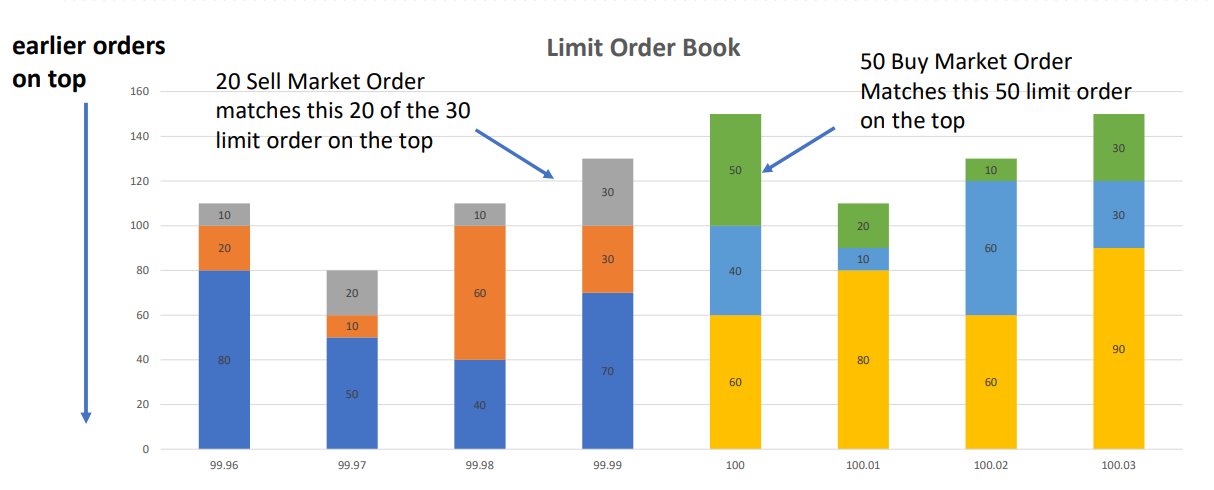
\includegraphics[scale=0.3]{img/limit_order_book.png}
    \end{center}

    The market makers profit off of the \textbf{bid-ask spread}, which is the difference in the buy and sell price. If a seller wants to sell at \$99.99 and a buyer wants to buy at \$100.00, then the market maker can buy the stock from the seller for \$99.99 and sell it to the buyer at \$100.00, making a \$0.01 profit. 

    We can also look at it from an economic perspective. We can draw the supply and demand curves for a certain company's stock. We can treat stocks as goods, with the company being the supplier and public investors as the consumers. 
    \begin{enumerate}
      \item The demand curve says: as the price for a stock, i.e. a piece of the company, increases the quantity demanded by the market (consumers) will decrease because the costs of buying the stock will outweigh the marginal value of the share. There is a very important distinction to make here between stocks and other type of goods. Unlike consumable goods which we can clearly observe a diminishing marginal value (drinking 1 can of soda vs 2 cans vs 3 cans vs...), stocks do not seem to have any diminishing marginal value. That is, if I buy 10 shares, I expect to get precisely 10 times the profit than if I bought just 1 share. The value is not diminishing, so why is the demand curve monotonically decreasing? That is because it is not diminishing \textit{for an individual}, but if we look at a market of many individuals, they all have different interpretations of what the marginal value of the stock is. Individual $A$ may interpret the marginal value as $\$10$, while $B$ sees it as worth $\$8$, and $C$ sees $\$6$. All three marginal utility curves would be horizontal, but if we take the market utility, we can see that it is decreasing (e.g. at the price of $\$7$, a share is attractive to $C$ but not $A, B$, and at $\$9$, a share is attractive to $B, C$ but not $A$). Buying an infinite number of shares is not realistic, so let us assume that each person has $\$25$ worth to invest. 
      \begin{center}
        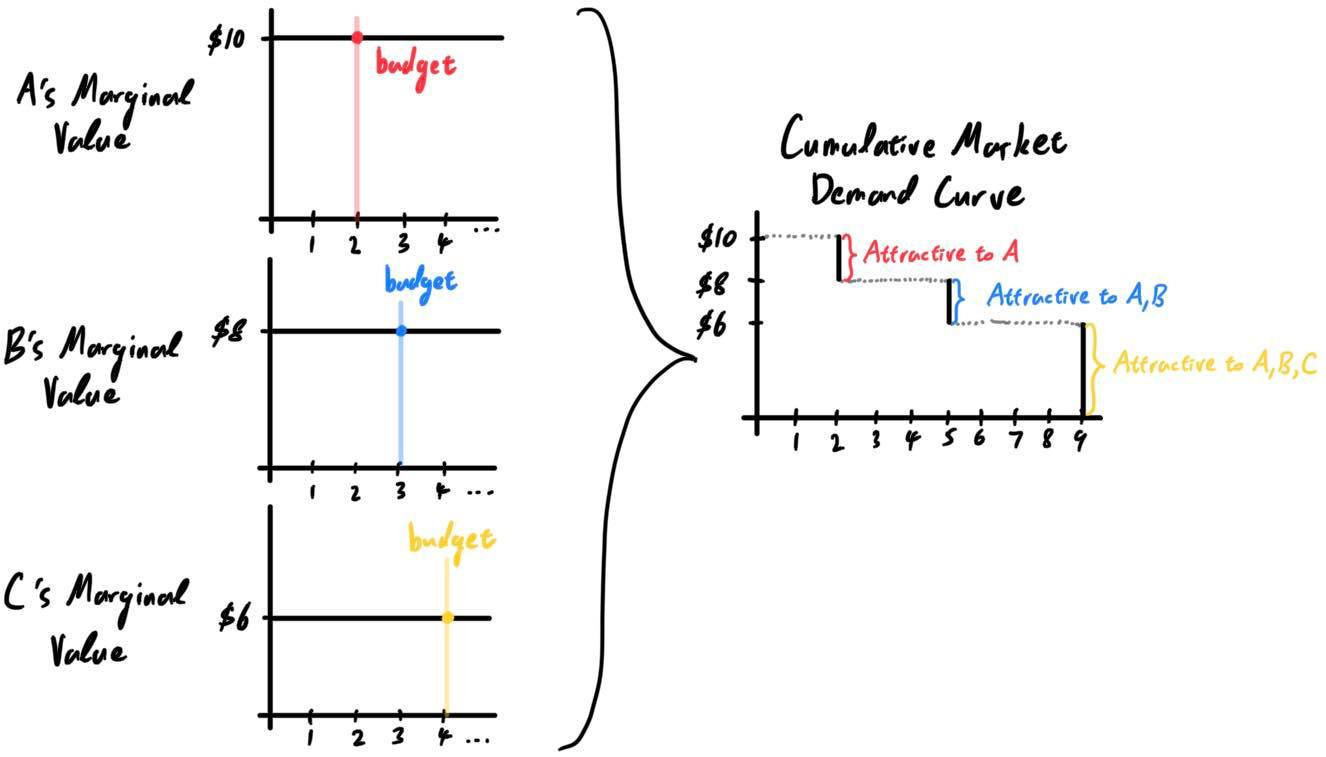
\includegraphics[width=0.8\textwidth]{img/Stock_demand_curve.jpg}
      \end{center}
      We can clearly see that the sum of these individual horizontal marginal value functions summed up produces a monotonically decreasing marginal value function and a monotonically decreasing demand curve for the total market. 

      \item The supply curve is simpler to interpret, since the only supplier is the issuing company (or whatever underwriting investment banks). By the law of supply, we can interpret that if the worth of the company's shares increases, then it would be logical for the company to issue more shares, all else being the same. This interpretation may be too oversimplistic, since we have to account for investor relations, dilution, and other factors, but it will do for now to justify that the supply curve of a stock is monotonically increasing.  
    \end{enumerate}

    Note that in general, the demand of a company's shares is much more volatile than the supply since there are many ways for the demand to shift, while few for the supply. The demand (not quantity demanded) of a company's shares can be changed from news, world events, production, and such, which occurs often and may even violently shift the outlook of the business. Unlike certain goods that are produced continuously, a company's floating shares will not change unless there is a new issuance or a private investors sells shares at market price. Therefore, supply (not quantity supplied) does not change easily. 

    Now, let us have the supply and demand curves of a company's share. Assume that it is at the equilibrium position, where $p^\ast_1$ is the current market price (bought and sold) and $q_1^\ast$ is the quantity demanded and supplied, as balance. 

    \begin{enumerate}
      \item If the demand increases, then the shift in the demand curve raises the equilibrium price to $p_2^*$, which raises the price of the stock. The quantity demanded/supplied also increases to $q_2^*$, but this desire to increase quantity cannot be met due to other factors. Therefore, we can interpret this case as such: The increase in demand can change the price accordingly, but the increase in desired quantity is offset by other factors (not being able to issue stocks freely). 
      \begin{center}
        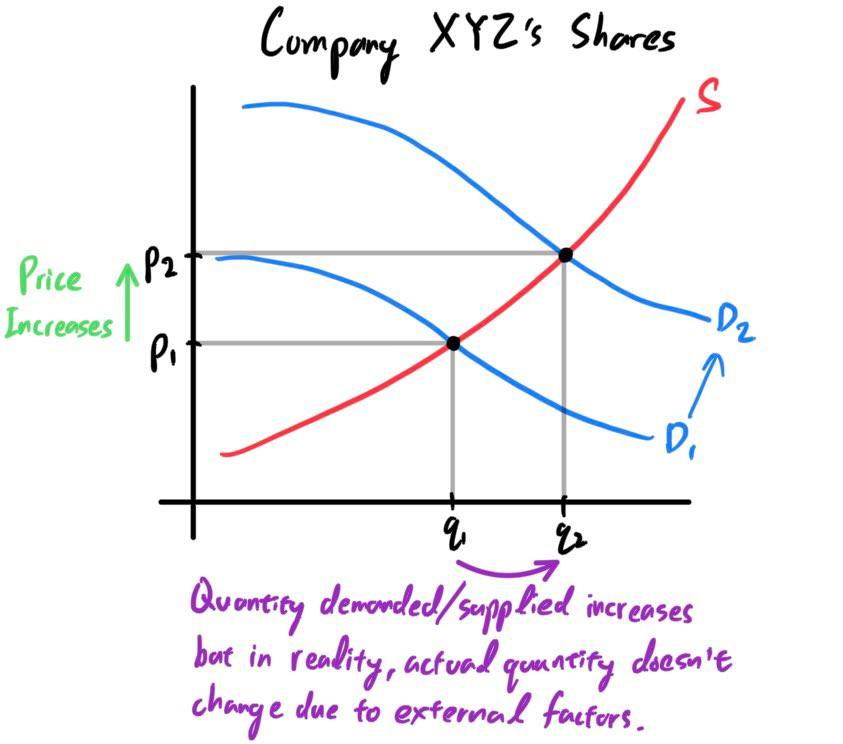
\includegraphics[width=0.4\textwidth]{img/Stock_Demand_Increase.jpg}
      \end{center}

      \item If the supply increases, then this is much simpler to explain. Due to dilution, one stock now represents ownership of a smaller portion of the company, driving the price down. The equilibrium (optimal) quantity demanded and supplied increases due to this higher supply, which is reflected in the reality that there are more more shares issued now. 
      \begin{center}
        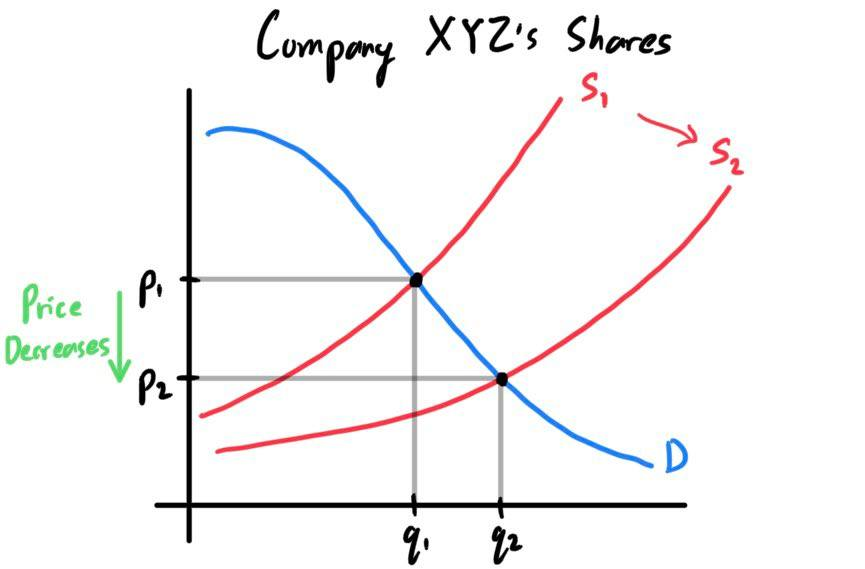
\includegraphics[width=0.4\textwidth]{img/Stock_Supply_Increase.jpg}
      \end{center}
    \end{enumerate}

  \subsection{Returns and Dividends}

    We can work out its return as the percentage increase or decrease of its price. But given that $X_t$ is close to $X_s$, we can look at the Taylor expansion of $\ln(X_t)$ to be 
    \begin{equation}
      \ln(X_t) \approx \ln(X_s) + \frac{1}{X_s} (X_t - X_s) \implies \frac{X_t - X_s}{X_s} \approx \ln (X_t) - \ln (X_s) = \ln \bigg( \frac{X_t}{X_s} \bigg)
    \end{equation}
    Therefore, we work with \textit{log returns} as an appropriate approximation of the return. 

    \begin{definition}[Log Return]
      The \textbf{log return}, or \textbf{return}, of a stock from time $s$ to $t$ is defined 
      \begin{equation}
        R_{s, t} = \frac{X_t - X_s}{X_s} \approx \log\bigg( \frac{X_t}{X_s} \bigg) = \log(X_t) - \log(X_s)
      \end{equation}
      However, the return is almost always annualized, so we just write the return as $R$. 
    \end{definition}

    It has its advantages: 
    \begin{enumerate}
      \item It is time-additive: If we have prices $X_r, X_s, X_t$ for $r < s < t$, we can see that 
      \begin{equation}
        R_{[i, j]} + R_{[j, k]} = \log \bigg(\frac{P_j}{P_i}\bigg) + \log \bigg( \frac{P_k}{P_j} \bigg) = \log \bigg(\frac{P_k}{P_i} \bigg) = R_{[i, k]}
      \end{equation}

      \item Symmetricity: It is well known that a stock going down $50\%$ and then going up $50\%$ does not return the stock to its original price, despite it "looking" like it did. This effect is killed when looking at log returns. If $X_t = X_s (1 - k)$ for $0 < k < 1$, then we know that it must scale up by a factor of $\frac{1}{1 - k} \neq 1 + k$ to get the original price. Indeed, it is clearly the case that 
      \[\log(1 - k) + \log(1 + k) = \log(1 - k^2) < 0\]
      and in fact is always less than $0$ (so we always lose money). This is due to the concavity of this function. 
      
      \item It focuses on relative change, which is typically invariant on the underlying price of the stock. 
    \end{enumerate}

  
    \begin{definition}[Dividend]
      Given time $s, t$ with $s < t$, the dividend that a stock $X$ pays within time interval $[s, t]$ is the random variable $D_{s, t}$
    \end{definition}

    \begin{definition}[Total Return]
      Given that you own stock $X$, the amount of money you would have made from time $s$ to $t$ is the random variable 
      \begin{equation}
        X_t - X_s + D_{s, t}
      \end{equation}
      The \textbf{total return} during that period is defined 
      \begin{equation}
        \mathbf{R}_{s, t} = \frac{X_t + D_{s, t} - X_s}{X_s} \approx \ln(X_t + D_{s, t}) - \ln (P_i)
      \end{equation}
      which is the price return plus the dividend rate. Again, the total return is almost always annualized.   
    \end{definition}

    These properties allow us to focus on the returns to calculate our metrics. 

    \begin{definition}[Expected Return]
      The \textbf{expected return} of a stock from time $s$ to $t$ is simply the expected value 
      \begin{equation}
        \mathbb{E}[R_{s, t}] = \mathbb{E} [ \log(X_t) - \log(X_s) ]
      \end{equation}
      where the expectation can be over the whole $\sigma$-algebra of sequences or can be conditioned on the two random variables $X_s, X_t$. The expected return over a year is $\mathbb{E}[R]$. 
    \end{definition}

  \subsection{Volatility}

    While we should be comfortable working with specific time periods $[s, t]$, most of the time we will be working with annualized statistics. Therefore, what we really just want to know is \textit{what kind of distribution is $R$ for a given stock?} It is also often (but probably incorrectly) assumed that $R$ just stays relatively the same random variable for a number of years. Therefore, everything boils down (for not) to accurately modeling $R$. The next best thing to do after the expectation is the second moment. 

    \begin{definition}[Volatility]
      The \textbf{volatility} of a stock is the standard deviation of $R$. 
      \begin{equation}
        \sigma = \sqrt{\mathrm{Var}[R]}
      \end{equation}
    \end{definition}

    \begin{definition}[Realized Volatility]
      Again, we don't know this actual value so we look at the next best thing: the sample volatility, known as the \textbf{realized volatility}. All realized volatility is again annualized, but the frequency and time periods that we look at it is important. 
      \begin{enumerate}
        \item The \textbf{historical (realized) volatility} takes into account the volatility of the past. 
        \item The \textbf{future realized volatility} is for the future. This is what everybody wants to know. 
      \end{enumerate}
    \end{definition}

    It seems that the most straightforward frequency and time for volatility is by taking all the yearly returns of every fiscal year up until now. This has the disadvantage of a small number of samples since most companies are publicly listed for at most a few dozen years.\footnote{Rather than taking samples $R_{0:365}, R_{366:730}, \ldots$, one might ask whether we can take $R_{0:365}, R_{1:366}, R_{2:367}, \ldots$. The answer is no, since these samples are correlated. } Therefore, people often resort to the following: 
    \begin{enumerate}
      \item 52-week volatility and scale it up by $\sqrt{52}$ to get the annual volatility.
      \item 250-day volatility and scale it up by $\sqrt{250}$ to get the annual volatility.
      \item 12-month volatility and scale it up by $\sqrt{12}$ to get the annual volatility.
      \item Minutely volatility is not really used. 
    \end{enumerate}
    This is known as the \textbf{square-root-of-time rule}. 

    \begin{figure}[H]
      \centering 
      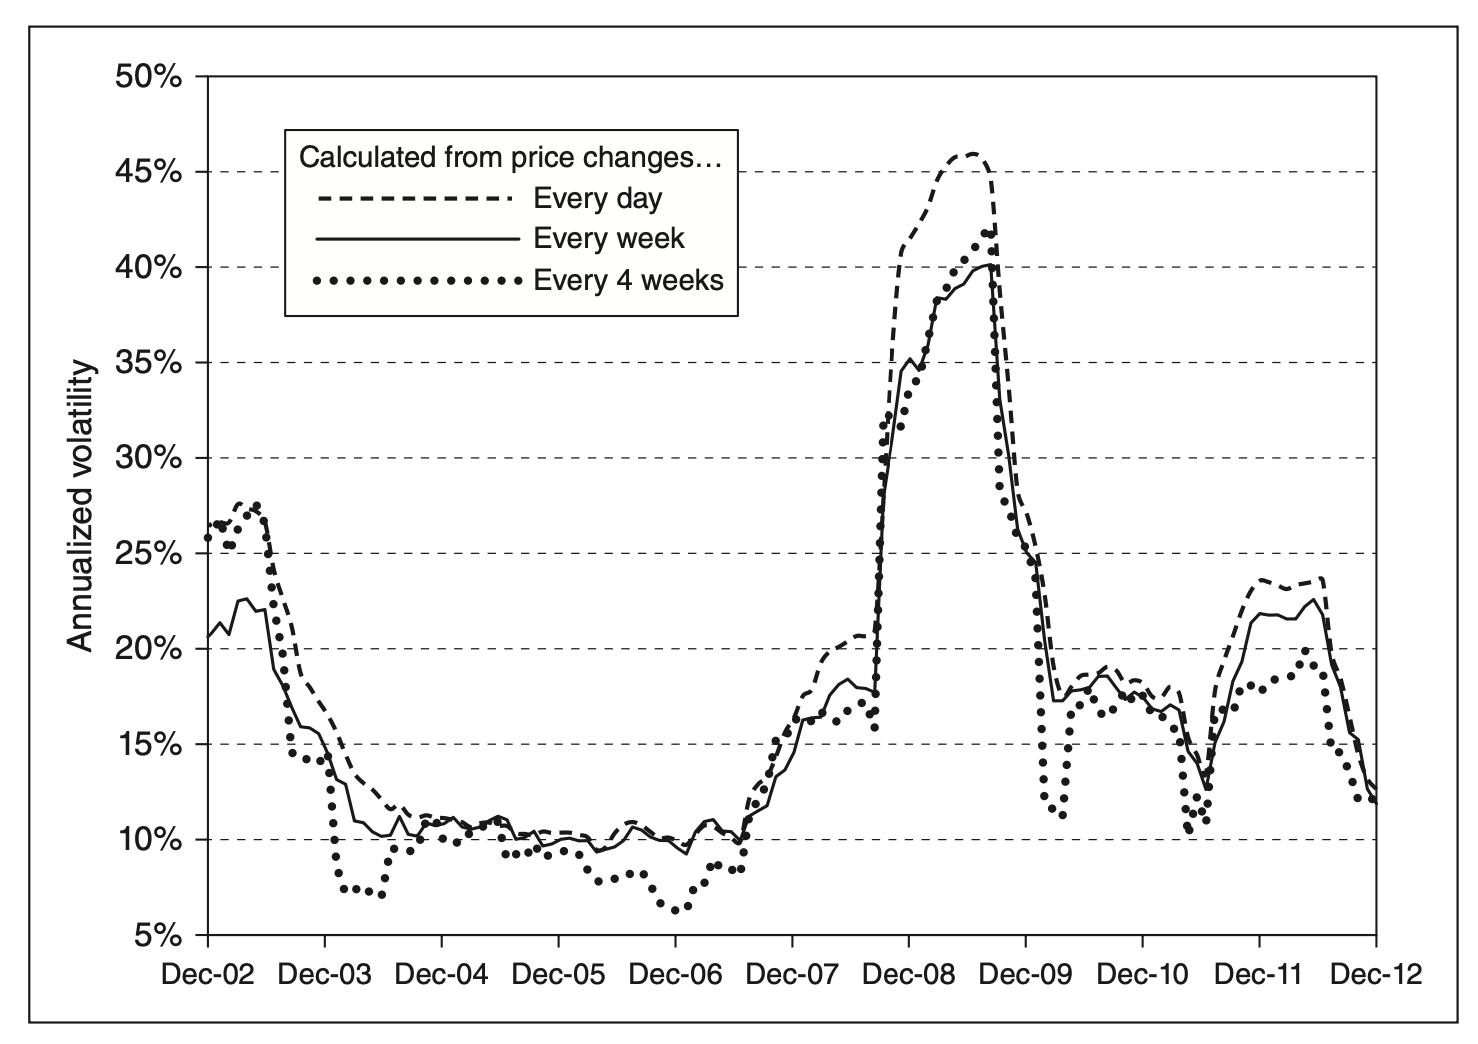
\includegraphics[scale=0.4]{img/vol_time_periods.png}
      \caption{The annaulized volatility over different time periods tend to be the same. } 
      \label{fig:volatility_time_periods}
    \end{figure}

  \subsection{Measures}

    While the expected returns are important, the concept of \textbf{risk} is equally if not more. This is a slippery term, used to mean different things, but it is essentially some characterization of the distribution of the returns. The variance, or standard deviation, of $R$ was one form of risk, but there are other ones that we will introduce here. 

    \begin{definition}[Sharpe Ratio]
      The \textbf{Sharpe ratio} is a measurement of risk-adjusted annual return. Given that you have some stock price with total return $R$ and volatility $\sigma$, the Sharpe ratio is defined as the random variable
      \begin{equation}
        S = \frac{R - R_f}{\sigma}
      \end{equation}
      where $R_f$ is risk-free return (e.g. the return you earn on U.S. Treasury bonds), which can be considered as a constant random variable. Sometimes, $R_f$ may not be constant and may be some time-series data itself. 
    \end{definition}

    Another property we would like to investigate is perhaps some tail bounds. 

    \begin{definition}[Value at Risk]
      The \textbf{value at risk (VaR)} over a time horizon of $T$ at $p \in [0, 1]$ is 
      \begin{equation}
        \Phi^{-1}(p)
      \end{equation}
      which tells us the loss we could incur by the end of $T$ with a probability of $p$, where $\Phi()$ is the CDF of $R_{0, T}$. $p$ is usually taken to be 1\% or 5\%. 
    \end{definition}

\section{Secondary Markets}

  \subsection{Types of Stock Orders}

    \begin{definition}[Stock Orders]
      The two most common orders one can do is the market order and the limit order. 
      \begin{enumerate}
        \item A \textbf{market order} just buys or sells securities at the market price. This ensures that the transaction will be completed, but the price at which you buy or sell may not be what you want. 
        \item A \textbf{limit order} buys or sells at least at a certain price. It ensures that you get the price you want for a transaction, but it may not be carried out always. 
        \begin{enumerate}
          \item A buy limit order at \$X tells the broker to buy a stock at \$X or lower. 
          \item A sell limit order at \$x tells the broker to sell a stock at \$ or higher. 
        \end{enumerate}
        \item A \textbf{stop loss order} is used to limit an individual's loss or lock in a profit on a stock position. 
        \begin{enumerate}
          \item If an investor buys a stock at \$100, they can make a stop loss at \$95. This means that when the stock price reaches \$95, then it will automatically place a market order to sell the stock (the price may not be fulfilled at exactly \$95 due to volatility). 
          \item If an investor has a short position, on the stock, then they can put a stop loss order at \$105, essentially telling the broker to buy the stock when the price reaches \$105. 
        \end{enumerate}
      \end{enumerate}
    \end{definition}

    \subsubsection{Short Selling}

      In addition to holding a long position, we can \textbf{short sell}, or short, a stock. Given that 100 shares of AAPL are each priced at \$100, we can borrow shares from some investor (probably an institutional investor), sell it on the market for \$100, and hope for the price to drop so we can buy it back. This is pretty symmetric to longing a stock, and many hedge funds use a \textbf{long-short equity strategy} involving a combination of longs and shorts, but there are additional risks. 
      \begin{enumerate}
        \item You must pay additional interest for borrowing stocks. 

        \item Your potential losses is not bounded. 

        \item If you have too much unrealized losses as the stock price goes up, then you may not have enough \textbf{margin} (cash) in your account to even buy back to stock. To prevent this, your broker may issue a \textbf{margin call}, which forces you to buy the stocks back, locking in your loss, unless you add more capital to your account. This margin call may not happen right at the point when your free cash is not enough to buy back all shorted shares. Rather, your brokerage may run some complicated statistical simulations, calculate some confidence interval, and then decide on a threshold that determines whether you will get a margin call. 
      \end{enumerate}
      The third risk is the deadliest, and at worst, you can get \textbf{short-squeezed}. Let's explain how this works. Say you and a bunch of other investors shorted GME. GME prices start going up, and it reaches a point where some investors have to buy back the GME shares due to a margin call. The investors buy back the GME at market price, which adds more orders to the limit order book, causing the price to go even higher. This higher price causes more short-sellers to buy back GME due to additional margin calls, causing GME to go even higher, and so on. This positive feedback loop is extremely deadly, killing off many short sellers. 

      Sometimes, the ethics of short selling are called into question. People who want to ban shorting state that short selling can drive down the stock price, which can be bad because it doesn’t spur the economy and reduces optimism in stock markets. Short selling means that stock is being borrowed and sold on the market, increasing supply, and therefore (all else being equal) decreasing price. However, these short sellers keep the stock price more in line with reality, and bad companies are punished by short sellers. 

      Finally, the entities that drive this short selling are \textbf{prime brokers}, which are large financial institutions (usually investment banks) that provide financial management to mainly hedge funds. They act on behalf of the short seller, locating the assets to be sold short for them and providing them with a margin account (which must hold capital to the sum of at least 150\% of the value of the initial transaction). They enable hedge funds to borrow large amounts of stocks from institutional investors to short-sell them and allow them to access large amounts of margin from commercial banks. The prime brokerage makes money through commissions. Prime brokers can also loan capital to investors to increase their leverage, and they also provide financial research and analytics to their clients. 

  \subsection{Counterparties and Clearing Houses}

    Trader, Broker, Liquidity provider, Market maker 

    NYSE is a stock exchange that leases a space to different market makers (banks, hedge funds). It also makes money thorugh fees from companies to be listed on NYSE. If a crash happens (i.e. a market maker buys a stock and it tanks before they can sell it), then the market makers get screwed. 

    Think about when one party buys stocks or bonds. Their downside is limited to the amount they paid on the stock, but there are many other cases where they may not be protected. 

    \begin{example}[Risks Associated with Trades]
      \begin{enumerate}
        \item The simplest case is when they are in debt. They want to borrow $X$ for a certain time, and repay it back in a year at some interest rate $X (1 + r)$. However, they may not have the money by then. 
        \item When they short a stock, they can borrow money from another party that owns the stock, sell it, and buy it back at a lower price. However, if the price of the stock rises, then they must pay even more money to buy it back, and they may not have enough money to. 
        \item When they buy a stock on margin, they borrow money from a broker to buy the stock, and they must pay back the broker with interest. However, the price of the stock may fall and the borrower, even after liquidating the stock, may not have enough money to pay back the broker.
        \item Someone who longs a forward contract may not have enough money to pay the difference between the forward price and the spot price.
      \end{enumerate}
    \end{example}

    \begin{definition}[Counterparty]
      A \textbf{counterparty} is the other party in a financial transaction. \textbf{Counterparty risk} is the likelihood or probability that one of those involved in a transaction might default on its contractual obligation. It can exist in credit, investment, and trading transactions.\footnote{This is formalized through creditworthiness, which takes many forms such as bond ratings, corporate credit ratings, and FICO scores.}
    \end{definition}

    Note that in a vanilla exchange, the two parties trading are counterparties to each other. This is called a \textbf{bilaterial exchange}. As we have seen, this is risky since if one party defaults, the other party is left with nothing. Therefore, the markets introduce a middleman that takes care of this risk. 

    \begin{definition}[Clearing House]
      The \textbf{clearing house} is an entity that is counterparty to all parties. This means that if party A and party B want to trade, they must go through the clearing house. The clearing house buys from B and sells to A. Therefore, the counterparty risk is now within the clearing house.
    \end{definition}

    It seems that we have simply moved the risk from the traders to the clearinghouse, and this is correct. The traders are glad that the risk is gone from them since they will always be paid by the clearinghouse, and the clearinghouse can add additional regulations on trading to reduce the risk of default. The first regulation they should impose are \textit{capital requirements}.\footnote{This is slightly different from margin. We will get to margin later. } 

    \begin{definition}[Capital]
      \textbf{Margin} is simply cash or some other asset (stocks, bonds, etc.) that can be used as collateral during a trade. Note that this does not mean that the collateral must be invested into anything. It is just restricted to sit there in your bank account. 
      \begin{enumerate}
        \item Cash is the most liquid form of margin, and is the most common form of margin. 
        \item Bonds are also a common form of margin, and Treasury bonds are usually valued at 90\% of their market value.
        \item Stocks are also a common form of margin, and are usually valued at 50\% of their market value. 
      \end{enumerate}
    \end{definition}

    Therefore, the cost of going into the trade is not just the trade itself, but also the capital requirements. These requirements are generally very inflexible unless you have a good relationship with your broker and are a big trader. 

  \subsection{Brokers}

  \subsection{Market Makers and Liquidity Providers}

  \subsection{Exchanges}

  \subsection{OTC Markets and Dark Pools}

    The inefficient aspect about markets that they are sensitive to large \textbf{block trades}, which are defined to be a trader involving at least 10,000 shares or at least \$200,000 (though they can get much larger). They are usually made by institutional investors and are often privately negotiated in order to prevent market price changes and fluctuations. When an institutional investor would like to make a sell block trade, they can either 

    \begin{enumerate}
      \item sell it on the exchange, where it will cause downwards pressure on the price, causing \textbf{slippage} (think of the limit order book: this sell order would clear out all buy orders past the sell price) and perhaps affecting the wider market. Even worse, once an order to sell a huge block has been filled, an investor can submit a buy order at a lower price in hopes that the block sell will hit his lowered price (this is an example of front running). 

      \item sell it privately off an exchange, but finding other parties to buy such a large amount is difficult. 
    \end{enumerate}

    Either way is quite unfavorable. The market impact of a sale of one million shares in Company XYZ could still be sizable regardless of which option the investor chose since it was not possible to keep the identity or intention of the investor secret in a stock exchange transaction. 

    These investors can trade in \textbf{dark pools}, which are privately organized financial exchanges for trading securities, also an \textbf{alternative trading system} (ATS). They were created originally to facilitate block trading by institutional investors who did not wish to impact the markets with their large orders. Most importantly, they keep trades anonymous. They allow traders to make block trades without having to publicize who they are, the buy/sell price, or the number of shares traded. 

  \subsection{Exchange vs OTC Markets}

    In a trading floor or pit, there are groups of traders huddled at certain physical locations that trade a certain asset, like corn futures. Back then, there would be individual traders that have their own small capital that they can trade with, called \textbf{locals}, but they have been dominated by traders that work for large financial institutions, causing locals to be either pushed our or joined with the firms. Market making firms like Akuna have pit traders, who have headsets and tablets, that are in real-time communication with the screen traders upstairs. 

    Standing in the perimeter of the trader circle are the \textbf{brokers}, who relay orders between the traders in the pit and outside of the pit. These brokers also have devices that allow them to communicate with \textbf{off floor} parties, who are individuals that are interested in these products. 

    \begin{example}[Off Floor Parties]
      Some examples of off floor parties are: 
      \begin{enumerate}
        \item Hedge funds, who have devised trading strategies that they want to implement, e.g. using drones to look at the harvest quantity. Now they want to gain exposure to the corn market. 
        \item Banks might also want to use client money to develop a trading strategy. 
        \item Consumers such as Kellogs (which needs a lot of corn to make cereal) might be interested in buying contracts to hedge their underlying exposure. 
        \item Producers like corn farmers might want to buy some contract to lock in the price in which they can sell it at. 
        \item Large funds like pension funds or family money. 
        \item Retail investors like small, non-professional traders that might dabble in options.  
        \item Other market makers might be connected to these brokers
      \end{enumerate}
    \end{example}

    Now if some off floor party decides to sell some calls, they will call their broker and ask to quote some prices. This means that they are asking for bid and offer prices. These traders might quote the following prices: 

    When more people want to buy and sell things, they must go to an \textbf{exchange}, which is literally a physical space that is leased to various parties (e.g. large banks, hedge funds) so that they can exchange goods. These exchanges also collect money through fees from companies to be listed on NYSE. There are two big exchanges, the NYSE and the NASDAQ, in the U.S., both located in New York. 

    Us retail traders are not direct participants of the exchange; the parties that participate there are called the \textbf{market makers}, or \textbf{liquidity providers}. Market makers, usually large banks or financial institutions (like hedge funds), make sure that there is enough trading volume to ensure liquidity in the market. A buyer and a seller must meet together to complete a deal, and to ensure that this happens smoothly (i.e. provides liquidity), a market maker buys stocks (through the individual's brokerage) and sells them to the corresponding recipient. Essentially, they provide a pool of shares and act as intermediaries between them. They profit from the bid-ask spread, though sudden volatility is always a risk. For example, if a crash happens (i.e. a market maker buys a stock and it tanks before they can sell it), then the market makers get screwed because they are left with an undervalued stock. 

    The trader cannot directly trade through the market makers. They must contact their \textbf{broker}, which is another company that acts as an intermediary. If I want to buy a stock, my buy order gets sent to my broker, which gets sent to the market makers, which pairs me up with a seller through their own broker, and the transaction is completed. These brokers make money through commissions from the traders and from trading in dark pools, which we'll talk about later. They also give access to traders the forecasts of analyst reports for companies and other research. 

    \begin{center}
      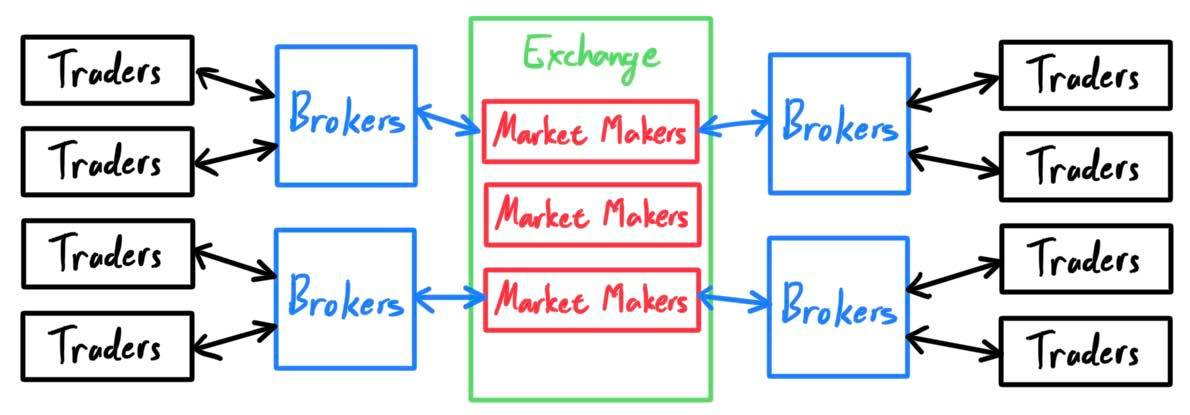
\includegraphics[scale=0.3]{img/exchange.jpg}
    \end{center}

    Clearly, there can be some shady stuff going on here, but luckily, the SEC and the FINRA consistently regulate the markets to ensure fairness for the little players (retail investors). One of the most important regulations is the 2005 Regulation NMS (National Market System), which required exchanges to publish the best bid and offer price for each stock, required them to route orders to the trading venue with the best price, and had set the minimal price quotation increment to \$0.01. This ensured transparency and protection of the investor with the best price execution (but this can be taken advantage of by high frequency traders). 

    \begin{definition}[Exchange Markets]
      \textbf{Exchange markets} are markets that exchange \textit{standardized} contracts and is \textit{highly regulated} (to protect investors) by a central authority. A buyer and seller come together to trade a contract, and they enter the contract through a \textbf{clearing house}, which is the \textit{counterparty} to all trades. That is, both the buyer and seller enter into a contract with the clearing house. Doing this reduces the counterparty risk by ensuring that both sides have adequate \textit{margin}. For example, if the buyer wins the bet and the seller can't pay, the clearing house will pay the buyer.
    \end{definition}

    \begin{question}
      Talk about counterparties, clearinghouses. 
    \end{question}

    \subsubsection{Market Making and High Frequency Trading}

      A significant mover of markets are \textbf{high frequency traders}, or HFTs. HFT is a type of algorithmic trading that are characterized by high speeds and high turnover rates. It is the primary type of algorithmic trading and consists of about 50\% of all equity trades in the U.S. There is an average of about 1 trader per 10 milliseconds. Whether HFT is beneficial is very controversial: 
      \begin{enumerate}
          \item Some argue that it is good since it increases liquidity and lowers transaction costs for retail investors. Even for potentially risky stocks (e.g. very overvalued), HFTs will always make a market out of them. 
          \item It can be considered unfair because it gives a huge advantage to HFT firms through front-running and other short-term strategies. This also increases the probability of \textbf{flash-crashes} (e.g. 2010 flash crash). 
      \end{enumerate}
      Unsurprisingly, many HFT firms are market makers due to their ability to provide liquidity. 

      The primary form of HFT is \textbf{scalping}, which profits off of small price changes. The multiple benefits and drawbacks are easy to spot: 
      \begin{enumerate}
          \item It requires a strict exit strategy since one large loss could eliminate the many small gains the trader worked to obtain. 
          \item It also requires a much higher ratio of winning trades vs losing ones, while keeping profits roughly equal or slightly bigger than losses. 
          \item A brief exposure to the market diminishes the probability of running into an adverse event like a crash. 
          \item Smaller moves are easier to obtain, so there are plenty of opportunities to exploit. 
      \end{enumerate}
      This strategy is extremely sensitive that even the physical location of the firm relative to the exchange matters. Heavy money in infrastructure is invested. 


    \begin{definition}[OTC Markets]
      In \textbf{over the counter markets} (OTC), there is also an interaction between the buyer and the seller, but it is done in two ways. 
      \begin{enumerate}
        \item In \textit{bilateral clearing}, the buyer and seller are the counterparties to each other, and so there is indeed the risk of default on one side. 
        \item Post-2008, there has been a push to clear through a \textit{central counterparty}. Therefore, there has been a slow push to clear OTC derivative trading to reduce this counterparty risk. 
      \end{enumerate}
      Finally, the OTC market is much larger (about 5 to 10 times larger in terms of the principal dollars underlying the assets) than the exchange and is less regulated since most of the players are institutional investors (they don't need as much protection but need more flexibility).  
    \end{definition}

\section{Momentum Strategies}

  Momentum strategies can be divided into \textbf{momentum trending}, which bets that the stock price will continue following the trend, and \textbf{momentum reversing}, which bets that the stock price will revert back to some mean. 

  \subsection{Moving Averages}

    The simple moving average and the exponential moving averages represent where the stock's price is at average. 

    \begin{definition}[Simple Moving Average]
      Let us have some stock price $\{P_i\}_{i=0}^N$ and fix some lookback parameter $L$. Then, the $L$-period \textbf{simple moving average (SMA)} of the stock is the average of prices of the past $L$ periods, $\{S_i\}_{i=L-1}^N$, where 
      \[S_i = \frac{1}{L} \sum_{j=i-L + 1}^i P_j\]
    \end{definition}

    \begin{definition}[Exponential Moving Average]

    \end{definition}

    We can build momentum strategies by comparing two different MAs of lookback periods $L_1 < L_2$. We can compare the current price to the moving averages, but the current price can be thought of as the $1$-period moving average anyways. The $L_2$-MA is thought of as the long term trend of the stock, while he $L_1$-MA is the short-term trend. The follow are essentially MA strategies. 
    \begin{enumerate}
        \item Momentum Trending: 
        \begin{enumerate}
            \item If the $L_1$-MA is above the $L_2$-MA, then the stock has momentum upwards. $\implies$ Long. 
            \item If $L_1$-MA is below the $L_2$-MA, then the stock has momentum downwards. $\implies$ Short. 
        \end{enumerate}
        
        \item Momentum Reversing: 
        \begin{enumerate}
            \item If the $L_1$-MA is above the $L_2$-MA, then the stock has momentum upwards. $\implies$ Short. 
            \item If $L_1$-MA is below the $L_2$-MA, then the stock has momentum downwards. $\implies$ Long. 
        \end{enumerate}
    \end{enumerate}

  \subsection{Bollinger Bands}

    \begin{definition}[Bollinger Bands]
      Let us have some stock price $\{P_i\}_{i=0}^N$ and fix some lookback parameter $L$, along with some $z$-score $Z$. We compute the standard deviation of the prices $P_i$ in the past $L$ periods to get $\{\sigma_i\}_{i=L-1}^N$. 
      \begin{enumerate}
        \item The \textbf{middle band} is defined to be the $L$-period SMA, which we will call 
        \[\{\mathcal{M}_i\}_{i=L-1}^N\] 
        \item The \textbf{upper band} is defined to be the band that is $Z$ standard deviations above the middle band. 
        \[\{\mathcal{U}_i\}_{i=L-1}^N = \{M_i + Z \sigma_i\}_{i=L-1}^N\]
        \item The \textbf{upper band} is defined to be the band that is $Z$ standard deviations below the middle band. 
        \[\{\mathcal{L}_i\}_{i=L-1}^N = \{M_i - Z \sigma_i\}_{i=L-1}^N\]
      \end{enumerate}
    \end{definition}

    Now the algorithm for Bollinger bands is very simple. 
    \begin{enumerate}
      \item In a momentum following case, if $P_i$ crosses below $\mathcal{L}_i$, we short, and if $P_i$ crosses above $\mathcal{U}_i$, we long. 

      \item In a momentum reversing case, if $P_i$ crosses below $\mathcal{L}_i$, we long, and if $P_i$ crosses above $\mathcal{U}_i$, we short. The upper band acts as a resistance level, and the lower band acts as a support level. 
    \end{enumerate}

  \subsection{Relative Strength Index}

    The relative strength index indicates the momentum or lack of it. 

    \begin{definition}[Relative Strength Index]
      Let us have some stock price $\{P_i\}_{i=0}^N$. Let us define the period changes as $\{D_i\}_{i=1}^N$ with $D_i = P_i - P_{i-1}$. Then, the total gain and total loss can be defined as 
      \[D_\mathrm{gain} = \sum_{D_i > 0} |P_i - P_{i-1}|, \;\;\; D_{\mathrm{loss}} = \sum_{D_i < 0} |P_i - P_{i-1}|\]
      Then, the \textbf{relative strength index (RSI)} is defined to be 
      \[RSI = 100 \, \frac{D_{\mathrm{gain}}}{D_\mathrm{gain} + D_{\mathrm{loss}}}\]
      which ranges in $[0, 100]$, where $0$ is extremely bearish and $100$ is extremely bullish. Roughly, the RSI being $30$ means that for every 1 increase in a period, there are 2 decreases in other periods. The RSI being $70$ means that for every 1 decrease, there are 2 increases. 
    \end{definition}

    The algorithm is quite simple: 
    \begin{enumerate}
      \item In a momentum following case, if the RSI is below $30$, we short, and if the RSI is above $70$, we long. 
      \item In a momentum reversing case, if the RSI is below $30$, we long, and if the RSI is above $70$, we short. 
    \end{enumerate}

  \subsection{Determining Momentum Trending or Reversing}

    Now how can we quantitatively decide whether we should use a momentum trending or reverting strategy? We can measure this behavior of a stock by looking at its autocorrelation. 

    \begin{definition}[Autocorrelation]
      Let us have some stock price $\{P_i\}_{i=0}^N$ and fix some lookback parameter $L$. We construct a lagged version $\{P_i\}_{i=0}^{N-L}$ and compute the correlation of this lagged time series with the original. 
      \[\mathrm{Corr}(\{P_i\}_{i=0}^{N-L}, \{P_i\}_{i = L}^{N})\]
      is called the $L$-period \textbf{autocorrelation} of the stock price. 
    \end{definition}

    We can determine which strategy to use as follows. Let us assume that $L$ is small.  
    \begin{enumerate}
      \item If this autocorrelation is high (near $1$), then this indicates that if the stock moves in a certain direction, it is likely to move in that same direction $L$ periods later. So we should use a momentum following strategy. 
      \item If it is negative (near $-1$), it indicates that if the stock moves in a certain direction, it is likely to move in the opposite direction $L$ periods later. So we should use a momentum reverting strategy. 
    \end{enumerate}
    Trend following stocks tend to be growth stocks, while trend reversing ones are the traditional conservative companies. 

\section{Statistical Arbitrage}

  Intuitively, pairs trading takes two stocks of very similar companies and bets that they will rise and fall together. If one rises and the other falls, then we can long the one that falls and short the one that rises, ultimately betting on the way that they will converge. Let's first look at an intuitive examples with temperature betting. 

  \begin{example}[Temperatrue Arbitrage]
    Say you are given the following trades:
    \begin{enumerate}
      \item 65 at 66 on the temperature of San Francisco, $S$
      \item 45 at 47 on the temperature in Kyiv, denoted $K$
      \item 25 at 26 on the temperature of San Francisco minus Kyiv, $S - K$ 
    \end{enumerate}
    What do you do? Let's compare these markets. You see that buying $K$ and $S - K$, which you can do for $47 + 26 = 73$ must be the same as buying $S$ alone, which is $66$. Therefore there is a price mismatch. You should therefore long $S$, short $K$, and short $S - K$. 
  \end{example}

  To do this, take two sets of stock prices $P_t$ and $Q_t$ and model them with the assumption that the log returns are linearly correlated by the following relationship.\footnote{What beginners assume is that if $P$ rises by $5\%$, then $Q$ will also rise by $5\%$. But what if companies $P$ and $Q$, who use the same supply chains, exist such that $P$ is, say twice as dependent as $Q$? Then, if $P$ goes down by $5\%$, then $Q$ may go down by $2.5\%$, and our assumption should be that it is \textit{linearly correlated}. }
  \begin{equation}
    \frac{\Delta P}{P} = \beta \frac{\Delta Q}{Q} \iff \log(P_j) - \log(P_i) = \beta \big( \log(Q_j) - \log(Q_i) \big)
  \end{equation}

  This results in the model 
  \begin{equation}
    \log(P) = \beta \log(Q) + \alpha + \epsilon
  \end{equation}
  which can be seen to be equivalent because taking the change over time $[i, j]$ on both sides gives 
  \begin{equation}
    \Delta \log(P) = \beta \Delta \log(Q) + \Delta \epsilon \iff \frac{\Delta P}{P} = \beta \frac{\Delta Q}{Q} + \Delta\epsilon 
  \end{equation}
  So, if we look at
  \begin{equation}
    \{\epsilon_i\}_{i=0}^n = \{\log(P_i) - \beta \log(Q_i) - \alpha\}_{i=0}^n 
  \end{equation}
  we expect this to be a $0$-mean time series. Let the standard deviation be $\sigma = \sigma(\{\epsilon_i\}_{i=0}^n)$ and let us fix some $Z$-score threshhold. Then 
  \begin{enumerate}
    \item If $\epsilon_i > Z \sigma$, then short $P$ and long $Q$. 
    \item If $\epsilon_i < -Z \sigma$, then long $P$ and short $Q$. 
  \end{enumerate}

  \subsection{Long/Short Market Weights}

    But how much should we long or short? Let's look at a couple scenarios: 
    \begin{enumerate}
        \item If $\beta = 1$, and we shorted $\$99$ of $P$ and long $\$1$ of $Q$, then a $5\%$ rise in $P$ would result in $5\%$ rise in $Q$, but since we shorted much more of $P$, we would have a net loss. To mitigate this risk, we should have a weight of $P:Q = 1:1$. 
        \item If $\beta = 10$, and we shorted equally $\$50$ of $P$ and long $\$50$ of $Q$, then a $10\%$ rise in $P$ would result in a $1\%$ rise in $Q$. But since we had equal weights in $P$ and $Q$, this scenario would cause 10 times more losses in $P$ than gains in $Q$, resulting in a net loss. To mitigate this risk, we should have a weight $P:Q = 1:10$. 
    \end{enumerate}
    So, we need to be careful of setting the ratio of our market weights of the stocks $P$ and $Q$: 
    \[\lambda = \frac{\MV_Q}{\MV_P}\]
    Intuitively, we can see that our ratio should be $1: \lambda = 1:\beta$, i.e. $\lambda = \beta$, but let's formalize this with some mathematical derivation. Our portfolio value is 
    \[V = \MV_P + \MV_Q\]
    where $\MV_P = n_P P$ and $\MV_Q = n_Q Q$, where $n_P, n_Q$ are the number of shares of $P, Q$. If we are longing $P$ and shorting $Q$, then $n_P > 0$ and $n_Q < 0$. Then, our change in portfolio value $V$ is 
    \begin{align*}
        \Delta \V & = \Delta \MV_P + \Delta \MV_Q \\
        & = \MV_P \bigg[\frac{\Delta \MV_P}{\MV_P} + \frac{\MV_Q}{\MV_P} \frac{\Delta \MV_Q}{\MV_Q}  \bigg] \\
        & = \MV_P \bigg[ \frac{\Delta P}{P} + \lambda \frac{\Delta Q}{Q} \bigg] \\
        & = \MV_P \bigg[ \beta \frac{\Delta Q}{Q} + \Delta \epsilon + \lambda \frac{\Delta Q}{Q} \bigg] \\
        & = \MV_P \bigg[ (\beta + \lambda) \frac{\Delta Q}{Q} + \Delta \epsilon \bigg] 
    \end{align*}
    Therefore, our change in portfolio value depends on the terms in the last equation. We don't want the change $\Delta Q$ to have any effect on the performance, so we set $\lambda = - \beta$, ultimately resulting in 
    \[\Delta \V = \MV_P \Delta \epsilon\]
    and now our performance is purely dependent on $\Delta \epsilon$. We would like $\Delta \V$ to be positive, so if we are longing $P$, i.e. $\MV_P > 0$, then we want $\Delta \epsilon$ to also be positive. Likewise, if we are shorting $P$, then $\MV_P < 0$ and so we want $\Delta \epsilon < 0$. 

  \subsection{Choosing Correct Stocks}

    So, how do we ensure that $\Delta \epsilon$ behaves this way? Remember that $\{\epsilon_i\}$ is $0$-mean time series. However, we want to impose the additional condition that it is \textit{mean-reverting} as well. That is, we don't want it to diverge or oscillate too frequently $\epsilon_i$, since if it did then there is the risk of $\{\log(P_i) - \beta \log(Q_i) - \alpha\}_{i=0}^n$ swinging too widely, resulting in losses. In other words, if $\epsilon_i > 0$, then we want $\Delta \epsilon_{i + 1} = \epsilon_{i+1} - \epsilon_i < 0$, and if $\epsilon_i < 0$, then $\Delta \epsilon_{i+1} > 0$, so that the $\epsilon_i$'s tend to "go back towards $0$." More formally, we can plot all $\epsilon_{i-1}$'s with the $\Delta \epsilon_i$'s, and look at a potentially linear relationship 

    \begin{equation}
      \Delta \epsilon_i = \alpha \epsilon_{i-1} + \xi_i
    \end{equation}

    To be mean reverting, we want to test that $\alpha < 0$ with adequate statistical significance, i.e. with p-value $5\%$. By looking at not just the previous $\epsilon_{i-1}$ but also the last $p$ $\epsilon_i$'s we can develop the general linear relationship 

    \begin{equation}
      \Delta \epsilon_i = \xi_i + \sum_{j=1}^p \alpha_j \epsilon_{i - j}
    \end{equation}

    This is called the \textbf{Augmented Dickey Fuller (ADF)} test, which tells us whether a time series is mean-reverting or not. 

\section{Portfolios}

  \begin{definition}[Portfolio]
    A \textbf{portfolio} is a collection of assets $X^{(1)}, X^{(2)}, \ldots, X^{(n)}$ with weights $\omega_1, \ldots, \omega_n$ s.t. $\sum \omega_i = 1$.\footnote{Since we can short stocks, the elements can be negative, but we should restrict this somehow since we don't want to allow unlimited shorting, which would require infinite margin. } 
    \begin{enumerate}
      \item The returns $\mathbf{R} = (R^{(1)}, \ldots, R^{(n)})^T$ of each component may be correlated, and the \textbf{portfolio return} is the random variable. 
        \begin{equation}
          R = \boldsymbol{\omega} \mathbf{R} = \sum w_i R^{(i)}
        \end{equation}

      \item The covariance matrix
      \begin{equation}
        \boldsymbol{\Sigma} = \mathrm{Cov}(\mathbf{R}) \coloneqq \begin{pmatrix} \mathrm{Var}(R_1) & \ldots & \mathrm{Cov}(R_1, R_K) \\ \vdots & \ddots & \vdots \\ \mathrm{Cov}(R_K, R_1) & \ldots & \mathrm{Var}(R_K) \end{pmatrix} 
      \end{equation}
      can be used to calculate the \textbf{portfolio variance} and \textbf{portfolio volatility}. 
      \begin{equation}
        \mathrm{Var}(R) = \mathbf{w}^T \boldsymbol{\Sigma} \mathbf{w} \implies \sigma_{\mathrm{port}} = \sqrt{\mathrm{Var}[R]}
      \end{equation}
    \end{enumerate}
  \end{definition}

  \begin{definition}[Alpha]
    The \textbf{alpha} of a portfolio with return $R$ compared to some market return $R_m$ is defined as 
    \begin{equation}
      \alpha \coloneqq \mathbb{E}[R_p - R_m] = \mathbb{E}[R_p] - \mathbb{E}[R_m]
    \end{equation}
  \end{definition}

  \begin{definition}[Beta]
    Beta is a measure of volatility. The \textbf{beta} of a stock compared to some market is defined 
    \begin{equation}
      \beta \coloneqq \rho_{pm} \frac{\sigma_p}{\sigma_m} = \frac{\mathrm{Cov}(R_p, R_m)}{\mathrm{Var}(R_m)}
    \end{equation}
    where $\rho_{pm}$ is the correlation between $R_m$ and $R_f$ and $\sigma$ represents the volatility of returns. 
    \begin{enumerate}
      \item If a stock has beta value of $1$, then its price activity is strongly correlated with the market (or the benchmark $B_j$). 
      \item A $\beta < 1$ means that the security is less volatile than the market. 
      \item A $\beta > 1$ means more volatile. 
      \item A negative $\beta$ indices that the stock is inversely correlated with the market. 
    \end{enumerate}
  \end{definition}

  \subsection{Markowitz Portfolio Theory - Mean Variance Portfolio}
    
    Consider $n$ securities $X_1, \ldots, X_n$, with returns $R_1, R_2$ iid. s.t. $\mathbb{E}[R_i] = \mu$ and $\Var[R_i] = \sigma^2$. Now within a one period market, consider the two portfolios, which have the same expected return, but have different variance.  
    \begin{enumerate}
      \item Portfolio A, with 100\% invested in stock 1: 
        \begin{equation}
          R_A = R_1 \implies \mathrm{Var}(R_A) = w_1 \mathrm{Var}(R_1) = \sigma^2 
        \end{equation}
      \item Portfolio B, an equi-weighted portfolio: 
        \begin{equation}
          R_B = \sum \frac{1}{n} R_i \implies \mathrm{Var}(R_B) = \mathrm{Var} \bigg( \frac{1}{n} \sum_{i=1}^n R_n \bigg) = \frac{1}{n^2} \sum_{i=1}^i \mathrm{Var}(R_i) = \sigma^2 / n
        \end{equation}
    \end{enumerate}
    The volatility of $B$ is much better, where the Sharpe goes up by a factor of $\sqrt{n}$ as we increase our number of independent stocks. The key word is independence, which may not be a realistic assumption. Regardless, this reduces down to an optimization problem over some constrained space $\Omega \subset \mathbb{R}^n$, where we must find the optimal weights $\mathbf{w} = (w_1, \ldots, w_n)$ that maximizes expected return for some amount of risk, or equivalently gives us the lowest volatility for some around of expected return. This solution is called the \textbf{risk-return efficient portfolio}. 
    \begin{equation}
      \arg \min_{\mathbf{w} \in \Omega} \mathrm{Var}(R_{\mathbf{w}}) = \arg \min_{\mathbf{w} \in \Omega} \frac{1}{2} \mathbf{w}^T \boldsymbol{\Sigma} \mathbf{w}
    \end{equation}
    We look at variants of this optimization problem that basically includes different constraints. 

    \begin{example}[Efficient Frontier without Risk-Free Asset]
      Let us put the constraints that the expected returns must be $p$ and that we must invest all of our money. This leads to 
      \begin{equation}
        \Omega = \{ \mathbf{w} \in \mathbb{R}^n \, | \, \mathbf{w}^T \boldsymbol{\mu} = p, \mathbf{w}^T \mathbf{1} = 1 \}
      \end{equation}
      The solution to this optimization problem is called the \textbf{Markowitz efficient frontier}, which traces out a hyperbola of the form 
      \begin{equation}
        \sigma^2_R = A p^2 + B p + C
      \end{equation}
      if we get rid of the $\boldsymbol{\omega}$ parameter. Here we randomly sample a bunch of $\mathbf{w}$'s from $[0, 1]^K$ (subject to the constraints, of course), construct the return of the portfolio $R_{\mathbf{w}}$, and then plot the points $(\mathbb{E}[R], \Var(R))$. We can see that none of the points ever cross the frontier. 
      \begin{center}
        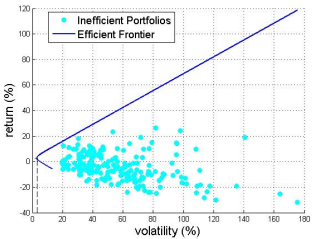
\includegraphics[scale=0.65]{img/Efficient_Frontier.png}
      \end{center}
    \end{example}

    \begin{example}[All Long Positions]
      Note that this efficient portfolio allows us to have unlimited short positions, which may or may not be realistic. If we wanted to work only with all-long portfolios, then we would impose the nonlinear restrictions 
      \begin{equation}
        0 \leq w_k \leq 1 \text{ for } k = 1, \ldots, K
      \end{equation}
      which would need to be solved numerically, possibly using nonlinear models. 
    \end{example}

    \begin{example}[Efficient Frontier with Risk-Free Asset]
      If we include a risk-free asset such as cash $C$ with risk-free return $R_f$ to the portfolio $\{P_1, \ldots, P_K\}$, then we slightly modify our equations. By definition, the risk-free asset has volatility $\sigma_0 = 0$ and its weight must be equal to $w_f = 1 - \sum_{i=1}^K w_k$
      , so we still want to minimize the same objective subject to constraint equations 
      \begin{equation}
        R_f \bigg( 1 - \sum_{k=1}^K w_k \bigg) + \sum_{k=0}^K w_k R_k = R
      \end{equation}

      When we allow our portfolio to include the risk-free security, the efficient frontier becomes a straight line that is tangential to the risky efficient frontier and with a $y$-intercept equal to the risk-free rate. 
      \begin{center}
        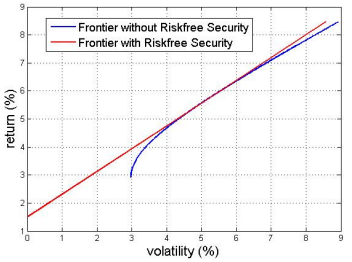
\includegraphics[scale=0.65]{img/Frontier_with_Risk_Free_Sec.png}
      \end{center}
      We can include other linear portfolio constraints, such as no-borrowing, no-short sales, or certain sector constraints. While analytic solutions are generally no longer available, the resulting problems are easy to solve numerically. 
    \end{example}

  \subsection{Capital Asset Pricing Model}

    Let us have some stock $P$ with random variable of return $R_p = R_{P, [i, j]}$ and the market $M$ with random variable of return $R_m = R_{M, [i, j]}$, both within period $[i, j]$. There may be some sort of risk-free return $r_f$ available (e.g. U.S. treasury bonds), so we can observe the returns of these two assets past the risk-free return by considering the joint distribution 

    \begin{equation}
      (R_p - r_f) \times (R_m - r_f)
    \end{equation}

    This may or may not be correlated, but the capital asset pricing model shows that there exists a linear relationship between the expected values of these two distributions. The central insight of the CAPM is that in equilibrium the riskiness of an asset is not measured by the standard deviation of its return but by its beta. 

    \begin{theorem}[CAPM]
      Now let $\overline{R}_m = \mathbb{E}[R_m]$ denote the expected return of the market, and $\overline{R} = \mathbb{E}[R]$ denote the expected return of a security or portfolio. Then, the \textbf{capital asset pricing model (CAPM)} asserts that there exists a linear relationship 
      \begin{equation}
        \overline{R} = r_f + \beta (\overline{R}_m - r_f)
      \end{equation}
      where $r_f$ is the risk-free rate. 
    \end{theorem}
    \begin{proof}
      Let us consider a portfolio of weights $\alpha$ and $1 - \alpha$ on the risky security and market portfolio, respectively. Let $R_\alpha$ denote the random return of this portfolio as a function of $\alpha$. We then have 
      \begin{align*}
          \mathbb{E}[R_\alpha] & = \alpha \overline{R} + (1 - \alpha) \overline{R}_m \\
          \mathrm{Var}(R_\alpha) & = \alpha^2 \mathrm{Var}(R) + (1 - \alpha)^2 \mathrm{Var}(R_m) + 2 \alpha (1 - \alpha) \mathrm{Cov}(R, R_m)
      \end{align*}
      Note that as $\alpha$ varies, the mean and standard deviation $(\mathbb{E}[R_\alpha], \mathrm{Var}(R_\alpha))$ trace out a curve in $\mathbb{R}^2$ that cannot cross the efficient frontier, as shown in the dotted line. 
      \begin{center}
          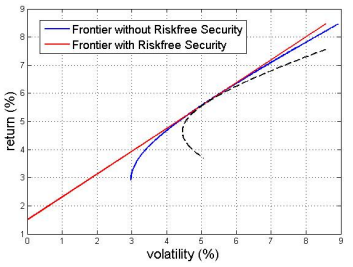
\includegraphics[scale=0.5]{img/CAPM.png}
      \end{center}
      At $\alpha = 0$, the slope of this curve must equal the slope of the capital market line. The slope of the $\alpha$-curve (where $\sigma(R_\alpha) = \sqrt{\Var(R_\alpha)}$) is 
      \begin{align*}
          \frac{d \mathbb{E}[R_{\alpha}]}{d \sigma(R_\alpha)} \bigg|_{\alpha = 0} & = \frac{d\mathbb{E}[R_\alpha]}{d \alpha} \bigg/ \frac{d \sigma(R_\alpha)}{d \alpha} \bigg|_{\alpha = 0} \\
          & = \frac{\sigma(R_\alpha) (\overline{R} - \overline{R}_m)}{\alpha \sigma(R) - (1 - \alpha) \Var (R_m) + (1 - 2 \alpha) \mathrm{Cov}(R, R_m)} \bigg|_{\alpha = 0} \\
          & = \frac{\sigma(R_m) (\overline{R} - \overline{R}_m)}{-\Var(R_m) + \mathrm{Cov}(R, R_m)}
      \end{align*}
      The slope of the capital market line is $(\overline{R}_m - r_f) / \sigma(R_m)$, and equating the two 
      \begin{equation}
        \frac{\sigma(R_m) (\overline{R} - \overline{R}_m)}{-\Var(R_m) + \mathrm{Cov}(R, R_m)} = \frac{\overline{R}_m - r_f}{\sigma(R_m)}
      \end{equation}
      gives the result. 
    \end{proof}

  \subsection{Efficient Market Hypothesis and No-Arbitrage Principle}

    \begin{definition}[Arbitrage Portfolio]
      A portfolio $\{X_i\}$ is an \textbf{arbitrage portfolio} if its current value $V^A (t) \leq 0$ and for some $T > t$, 
      \begin{enumerate}
        \item $V^A (T) \geq 0$ for all states of the world, with 
        \item $V^A (T) > 0$ with nonzero probability. 
      \end{enumerate}

    \end{definition}

    \begin{theorem}[Axiom of No Arbitrage]
      There exists no arbitrage portfolios, i.e. there is no free lunch. 
    \end{theorem}

  \subsection{Replication Principle}

    \begin{theorem}[Replication Principle]
      If we have two portfolios that have equal value at one point in time. Then they should have equal value at every other point in time. 
    \end{theorem}

\section{Derivatives}

  \begin{definition}[Derivatives]
    A \textbf{derivative} is a financial instrument whose value depends on (is \textit{derived} from) the value of some other, more basic, underlying variable. Essentially, given some stochastic process $X_t$ describing some variable, the derivative is some function 
    \begin{equation}
      Y_t = g(X_t)
    \end{equation}
    The reason that we say an underlying \textit{variable} is that it includes real assets (e.g. property), financial assets (e.g. stocks), indices (stock, inflation, or housing price index), or an event (e.g. weather, or the amount of rainfall in a given season to hedge against a bad winter). Therefore, these variables can be anything, like the number of people attending a fair, which may be an indicator of the profit of the fair or some catastrophic event, and we can derive value out of that event. Therefore, the variable does not necessarily have to be an asset. 
  \end{definition}

  \begin{example}[Weather Derivatives]
    A weather derivative can have payout of $g(S_T)$, where 
    \begin{equation}
      g(S_T) = \mathbbm{1} \{S_T > 50\} = \begin{cases} \$1 & \text{ if } S_T > 50 \\ 0 & \text{ if else} \end{cases}
    \end{equation}
    where $S_T$ is the total snowfall in inches during the year up to $T = 1$. Note that both $S_T$ and $g(S_T)$ are random variables whose value is unknown until $T = 1$.
  \end{example}

\section{Forwards and Futures} 

    Now we will see the most common type of derivative: the forward contract. 

    \begin{definition}[Forward Contracts]
      \textbf{Forward contracts} are contracts between two parties to buy or sell an asset at a future date for a price agreed upon today. For notation, let's write
      \begin{enumerate}
        \item $T$ is the time until delivery, usually in years. This is fixed per contract.
        \item $K$ is the delivery price. This is also fixed per contract. 
        \item $S_t$ is the spot price of the asset at time $t \in [0, T]$.
      \end{enumerate}
      A \textbf{future contract} is pretty much the same thing, except that it is traded on exchanges and is future-settled. 
    \end{definition}

    \begin{definition}[Value]
      Let $V_{K} (t, T)$ be the \textbf{true value} of the contract at current time $t \leq T$ of being long a forward contract with delivery price $K$ and maturity $T$. 

      The \textbf{price} is a noisy estimate of $V$. Let $P_t$ be the price of a long forward. 
    \end{definition}

    Note that $V_{K, T}$ is what everyone wants to find out but is extremely difficult. However, there are some properties that it must satisfy. 

    \begin{lemma}[Value at Maturity, Payout]
      Since the party that longs the forward contract must pay $K$ at $T$ to buy an asset which is worth $S_T$, the value of the contract at $T$ is 
      \begin{equation}
        V_K (T, T) = S_T - K
      \end{equation}
      This is referred to as the \textbf{value at maturity} or the \textbf{payout} of the contract.
    \end{lemma}

    \begin{example}[Red Sox]
      If I buy the Boston Red Sox regular season wins at 100, in size one dollar per won, I have a long forward position with delivery price of 100. If the Red Sox wins 110 games I make \$10, and if they have 91 wins I lose \$9. The payout is $S_T - K$ where $S_T$ is the number of wins. 
      \begin{figure}[H]
        \centering 
        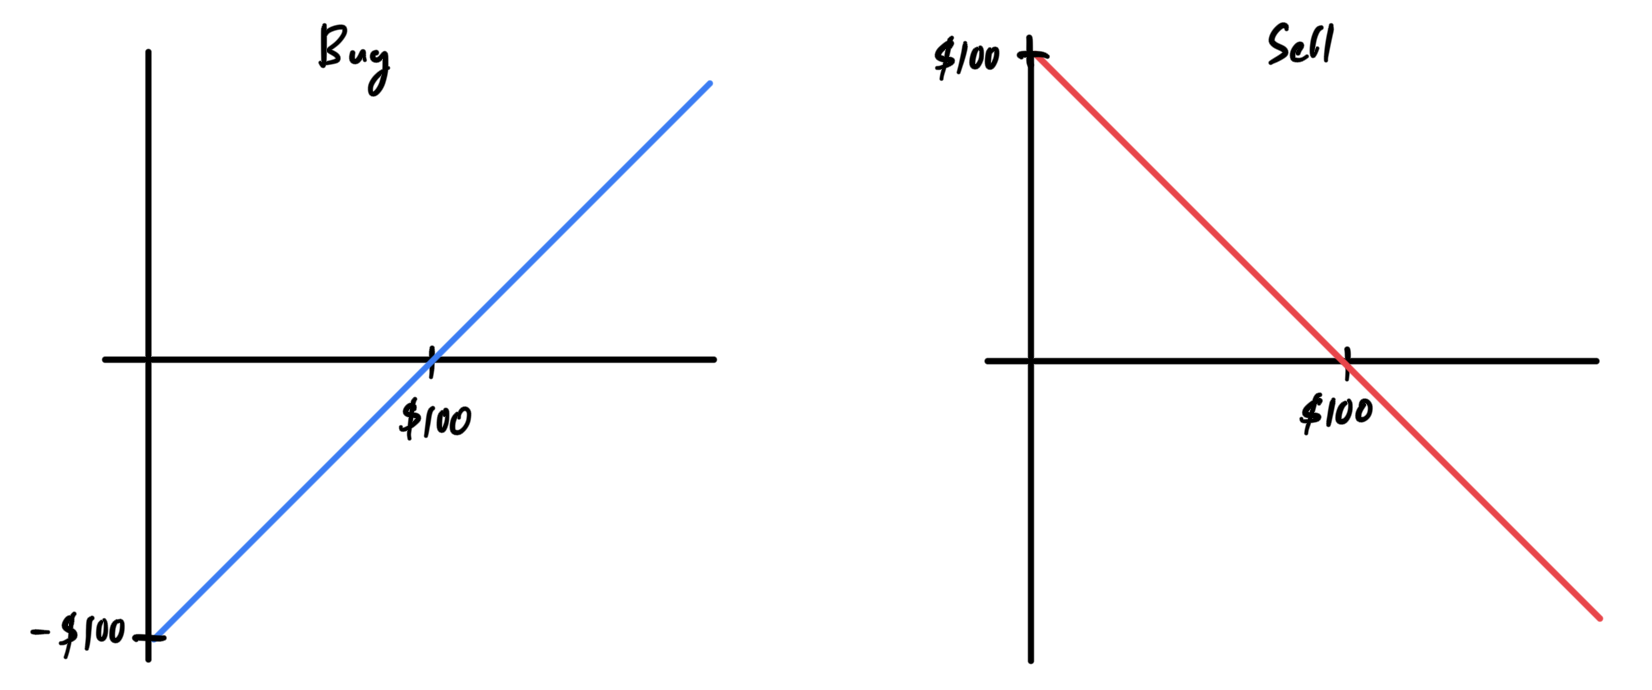
\includegraphics[scale=0.4]{img/forward_example.png}
        \caption{Payoff (not profit-loss) graphs for the buyer and sellers of the Red Sox contract. } 
        \label{fig:foward_example}
      \end{figure}
    \end{example}

  \subsection{Forward Price}

    When A and B enter into a forward contract, it should be the case that the value of this contract should be $0$ when both parties agree to it. To see why, consider the following equivalent scenarios between parties A and B, with interest rates being 10\%.\footnote{Thanks to \href{https://www.quora.com/Why-is-the-initial-value-of-a-forward-contract-set-to-zero}{this Quora post} for clarifying. } 

    \begin{enumerate}
      \item \textbf{A} must buy some product at \$400 from \textbf{B} in 1 year, which has a value of $0$ for both parties.  
      \item \textbf{A} must buy some product at \$300 from \textbf{B} in 1 year \textit{and} \textbf{A} must give \textbf{B} \$90.91 now (present value of \$100 in 1 year). The forward itself has positive value for \textbf{A} and negative value for \textbf{B}. 
      \item \textbf{A} must buy some product at \$500 from \textbf{B} in 1 year \textit{and} \textbf{B} must give \textbf{A} \$90.91 now. The forward itself has positive value for \textbf{B} and negative value for \textbf{A}. 
    \end{enumerate}
    Note that the second and third points are the same as initiating a $0$-value forward contract plus a separate loan. In scenario 2, \textbf{A} is loaning \textbf{B} \$90.91, which means that \textbf{A} is expected to receive \$100 and pay \$400 for the product, which is equivalent to paying \$300 for the product. This goes for scenario 3, where \textbf{B} now loans \textbf{A} \$90.01. 

    While this fact was obvious from the start, this scenario really emphasizes that the delivery price, along with the time period and interest rates, is a huge determinant in the value of the forward. A lower delivery price means positive value to the buyer (and negative to seller), and a higher delivery indicates positive value to the seller (and negative to buyer). \footnote{Depending on the buyer and seller's estimates of the interest rates, these may differ, but for now we assume one true rate. }The specific price where this value is $0$ is called the \textit{forward price}.

    \begin{definition}[Forward Price]
      The \textbf{forward price} $F(t, T)$ at the current time $t \leq T$ is the delivery price $K$ such that 
      \begin{equation}
        V_K (t, T) = 0 \implies V_{F(t, T)} (t, T) = 0 
      \end{equation}
      That is, it is the price that makes the contract have zero value at the current time. 
    \end{definition}

    \begin{lemma}[Forward Price at Expiry]
      By definition, it must be the case that $F(T, T) = S_T$ since to buy an asset at $T$ for the price $F(T, T)$ is the same as buying the asset at the spot price $S_T$. 
    \end{lemma}

    When the forward is created, it has no intrinsic value, but as time goes on, the value of the contract changes as the spot price changes. So if you find that the strike is greater than the forward price, then the person who longs that contract would have to buy at a high price, meaning that the value is negative. Otherwise it is positive. 

    \begin{example}[Constant Stock]
      Suppose that a stock which pays no dividends always has price $100$ and interest rates are always $0$. Then 
      \begin{enumerate}
        \item $F(t, T) = 100$ since if you had the right to buy the stock at $100$ at any time $T$, then this would be the same as buying the stock at the spot market, but it is always $100$ in the spot market. So the value of this contract must be $0$ for all $T$. 
        \item $V_K (t, T) = 100 - K$ since if you have the right to buy the stock at $K$ in time $T$, the spot price will always be worth $100$ so you're really gaining $100 - K$. Therefore the value of this contract must be $100 - K$ for all $T$. 
      \end{enumerate}
    \end{example}

    To try valuing forward contracts through some formula, we should have an analogous formula for forward prices. Essentially, the fair value of our forward price should be captured in this formula.  
    \begin{align*}
      \text{forward price } = \text{current spot price of underlying} & + \text{benefits of buying later} \\ 
                                                                       & - \text{costs of buying later}
    \end{align*}
    Let's think about the benefits of buying later, which is equivalent to the costs of buying now. 
    \begin{enumerate}
      \item \textit{Interest on Cash.} You can get interest on the cash you have now.  
      \item \textit{Inventory Costs.} There are inventory costs that you would incur from storing products, e.g. commodities. There are also transportation and insurance costs.  
    \end{enumerate}
    The benefits of buying now, or the costs of buying later, is as such: 
    \begin{enumerate}
      \item \textit{Convenience Yield.} The buyer may urgently need the product now to capitalize on some immediate business opportunity. 
      \item \textit{Fixed Income Payments.} By not owning a dividend-paying stock or bond now, you will miss out on fixed-income payments like dividends or coupon payments. 
    \end{enumerate}
  
    This leads to an interesting categorization of these markets. 

    \begin{definition}[Cotango, Backwardation Market]
      A futures market is said to be in 
      \begin{enumerate}
        \item \textbf{cotango} if forward prices are above spot prices: $F(t, T) > S_t$. 
        \item \textbf{backwardation} if forward prices are below spot prices: $F(t, T) < S_t$. 
      \end{enumerate}
      Cotango markets are known to be the default, while backwardation is a bit rarer. But for both markets, it must be the case that the spot and forward prices converge as $t \rightarrow T$. 
      \begin{figure}[H]
        \centering 
        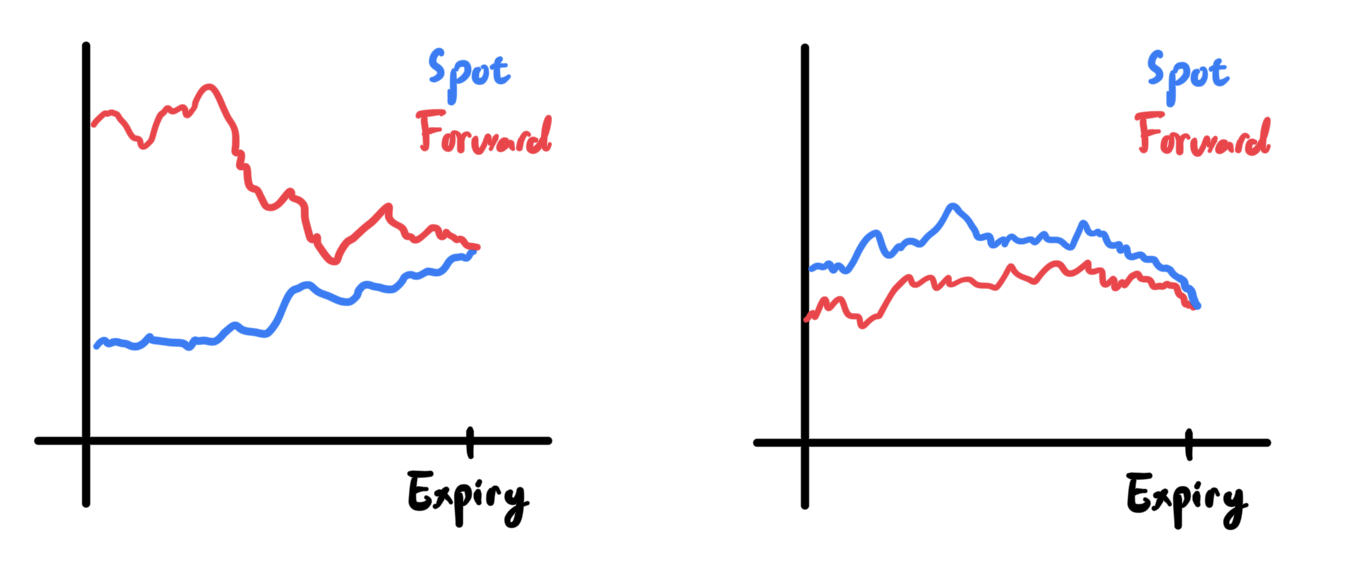
\includegraphics[scale=0.5]{img/cotango_backwardation.png}
        \caption{Spot and forward prices must converge upon expiry. If this wasn't the case, then we can construct an arbitrage pairs trade at expiry with the underlying and its forward contract. } 
        \label{fig:cotango_backwardation}
      \end{figure}
    \end{definition}

    Now we want to put this formula in more mathematical terms. Let's do this for underlying assets that gradually increase in complexity. 

    \begin{theorem}[Forward Price of No Income Asset]
      For an asset paying no income (e.g. a stock with no dividends), the forward price is 
      \begin{equation}
        F(t, T) = S_t e^{r (T - t)} \implies F(0, T) = S_0 e^{r T}
      \end{equation} 
    \end{theorem}
    \begin{proof}
      \textbf{Replication}. At current time $t$, let's take two portfolios. 
      \begin{enumerate}
        \item A: Consists of one unit of the underlying stock. 
        \item B: One long forward contract with delivery price $K$, plus $K e^{-r(T - t)}$ of cash. 
      \end{enumerate}
      At time $T$, B can invest the cash at the risk free rate $r$ and get $K$ cash. Then, it executes the forward contract at $K$ to get one stock. Therefore, at time $T$, both portfolios are worth $S_T$ and the values of both portfolios at time $t$ must also be the same. This is called the \textit{replication proof}. 
      \begin{equation}
        S_t = V_K (t, T) + K e^{-r (T - t)} \implies V_K (t, T)= S_t - K e^{-r (T - t)}
      \end{equation}
      We want to find the value of $K$ such that the value of the contract is $0$. Therefore, 
      \begin{equation}
        0 = S_t - K e^{-r (T - t)} \implies K = S_t e^{r (T - t)}
      \end{equation}
    \end{proof}
    \begin{proof}
      \textbf{No Arbitrage}. Another way to prove this is with the \textbf{No-arbitrage principle}. What we do is assume that the forward value is above or below our stated value, and prove that under these assumptions there is an arbitrage opportunity. 
      \begin{enumerate}
        \item Assume that $F(t, T) < S_t e^{r (T - t)}$. Then, you can buy a forward contract at delivery price $K = F(t, T)$ for free. You can also short the underlying stock at $S_t$ and invest the proceeds at the interest rate $r$. At time $T$, you can take your money, which is now worth $S_t e^{r (T - t)}$ and execute the contract by buying one share of the stock for $K = F(t, T)$. This leaves you with no stocks and money of $S_t e^{r (T - t)} - F(t, T) > 0$ by assumption, and you have an arbitrage opportunity.
        \item Assume that $F(t, T) > S_t e^{r (T - t)}$. Then, you can sell a forward contract at delivery price $K = F(t, T)$ for free. I borrow $S_t$ money at the interest rate $r$ and buy a stock. At time $T$, I sell the stock at $F(t, T)$ and also must pay back from who I borrowed at a rate of $S_t e^{r (T - t)}$. Therefore, this leaves me with a net gain of $F(t, T) - S_t e^{r (T - t)} > 0$ by assumption, and I have an arbitrage opportunity.
      \end{enumerate}
      Therefore, since I have an arbitrage opportunity, it must be the case that $F(t, T) = S_t e^{r (T - t)}$.
    \end{proof}

    Intuitively, with the no arbitrage strategy, we can see that if the forward price is too high relative to the stock price $S_t$, we buy the stock now and sell the contract (sell the stock forward at the higher price). If the forward price is too low, then we sell the stock now and buy the contract (buy the stock forward at the cheaper price). 

    \begin{corollary}[Dependence on Forward Price]
      The forward price is only dependent on the current underlying price $S_t$, the interest rate $r$, and the time to maturity $T - t$. Counterintuitively, it does not depend on the growth rate, the standard deviation, or any distributional assumptions of $S_T$. Furthermore, any two assets which pay no income and which have the same spot price $S_t$ will have the same forward price regardless of any views about their future movements. 
    \end{corollary}

    However, this is unrealistic in a few things. It first does not account for dividends, the cost of storage, or the cost of carry. 

    \begin{theorem}[Forward Price of Income Asset]
      Suppose an asset pays a known amount of income (e.g. dividends, coupons, rent) during the life of the forward contract and the present value at $t$ of the income is $I$. Then, 
      \begin{equation}
        F(t, T) = (S_t - I)e^{r(T - t)}
      \end{equation}
    \end{theorem}
    \begin{proof}
      \textbf{Replication}. Let us have two portfolios. 
      \begin{enumerate}
        \item A: Consists of one unit of the underlying stock. 
        \item B: Consists of one long forward contract with delivery price $K$, plus $K e^{-r(T - t)} + I$ of cash. 
      \end{enumerate}
      Then, B will invest the cash at the risk free rate $r$ and get $K + I e^{r(T - t)}$ cash. Then it uses $K$ to buy the underlying stock, ending up with $I e^{r(T - t)}$ in cash and one unit of stock. A, by owning the stock throughout the span, also receives $I$ of cash (present value), which is equal to $I e^{r(T - t)}$ worth at time $T$. Therefore, the two portfolios are equal at time $T$ and therefore must be equal at time $t$. 
      \begin{equation}
        S_T + I e^{r(T - t)} = V_K (T, T) + K + I e^{r(T - t)} \implies S_t = V_K (t, T) + K e^{-r(T - t)} + I
      \end{equation}
      Therefore, we can solve for the forward price by setting $V_K(t, T) = 0$. 
      \begin{equation}
        S_t = K e^{-r(T - t)} + I \implies F(t, T) = K = (S_t - I) e^{r(T - t)}
      \end{equation}
    \end{proof}
    \begin{proof}
      \textbf{No Arbitrage}. We assume the two scenarios. 
      \begin{enumerate}
        \item $F(t, T) < (S_t - I) e^{r(T - t)}$. Then, we buy the forward contract for free at $K = F(t, T)$ and short the stock at $S_t$. We take the proceeds of the short and invest it at the risk free rate $r$. At time $T$, we buy back the stock at $F(t, T)$, and give back the stock to the lender, and additional pay them the dividends they would have received, which is $I e^{r(T - t)}$. Therefore, our net profit is
          \begin{equation}
            S_t e^{r(T - t)} - F(t, T) - I e^{r(T - t)} > 0
          \end{equation}
        \item $F(t, T) > (S_t - I) e^{r(T - t)}$. Then, we buy the stock at $S_t$ and short the forward contract at $K = F(t, T)$ for free. At time $T$, we get our income $I e^{r(T - t)}$, pay back the lender at $S_t e^{r(T - t)}$, and execute the contract to sell it at $F(t, T)$. Our net profit is 
          \begin{equation}
            F(t, T) + I e^{r(T - t)} - S_t e^{r(T - t)} > 0
          \end{equation}
      \end{enumerate}
      Therefore, we have an arbitrage opportunity in both cases, and therefore it must be the case that $F(t, T) = (S_t - I) e^{r(T - t)}$.
    \end{proof}

    If the stock pays some income at a compounded rate, then we have the following result on the forward price. 

    \begin{theorem}[Forward Price of Compounded Income Asset]
      If the stock pays a continuous dividend yield $q$ (e.g. $q = 0.02$ means that the stock pays $2\%$ of its value in dividends each year), then the forward price is 
      \begin{equation}
        F(t, T) = S_t e^{(r - q)(T - t)}
      \end{equation}
    \end{theorem}

    At this point, we can take any financial security and interpret the forward price of it as the fair price of it at some predetermined point in the future. 

    \begin{example}[Forward Price of Commodities]
      The forward price of a commodity is 
      \begin{equation}
        F(t, T) = S_t (1 + r (T - t)) + s (T - t) + i (T - t)
      \end{equation}
      where $s, i$ are the annual storage, insurance costs per commodity unit.\footnote{This assumes no compound interest (?) } If these values are known, you can use them to predict other variables like the potential convenience yield. 
    \end{example}

    \begin{example}[Forward Price of Dividend-Paying Stock]
      Let 
      \begin{enumerate}
        \item $S_t$ be the stock price 
        \item $r$ be the interest rate over the life of the forward contract 
        \item $d_i$ is each dividend payment expected prior to maturity of the forward contract 
        \item $t_i$ is the time remaining to maturity after each dividend payment. 
        \item $r_i$ the applicable interest rate (i.e. \textit{forward rate}) from each dividend payment to maturity of the forward contract. 
      \end{enumerate}
      Then, the forward price of a dividend-paying stock can be written as the cash plus all the dividend payments, plus their interest. 
      \begin{equation}
        F(t, T) = S(1 + r (T - t)) - \sum_{i} d_i (1 + r_i t_i)
      \end{equation}
    \end{example}

    \begin{example}[Forward Price of Bond]
      Let 
      \begin{enumerate}
        \item $r$ be the interest rate over the life of the forward contract 
        \item $c_i$ be each coupon expected prior to the maturity of the forward contract 
        \item $t_i$ be the time remaining to maturity after each coupon payment 
        \item $r_i$ be the applicable interest rate from each coupon payment to maturity of the forward contract
      \end{enumerate}
      Then, the forward price of a bond can be written as 
      \begin{equation}
        F(t, T) = B(1 + r(T - t)) - \sum_i c_i (1 + r_i t_i)
      \end{equation}
    \end{example}

    Now we will make a bit of a loop here. What is the forward price of a futures contract? A futures contract is a forward contract, and it itself should have some fair price.  

    \begin{example}[Forward Price of Futures Contract]
      The forward price of a futures contract is the futures price. (?)
    \end{example}

  \subsection{Valuation}

    Recall from our example of the asset that pays no income. The replication argument gave 
    \begin{equation}
      S_t = V_K (t, T) + K e^{-r (T - t)}
    \end{equation}
    If we substitute $F(t, T) = S_t e^{r (T -t)}$ (that is, the forward price is the spot price compounded at the risk free rate), then we get
    \begin{equation}
      V_K (t, T) = (F(t, T) - K) e^{-r (T - t)} 
    \end{equation}
    which is the difference between the forward price and the delivery price, discounted back to today. 

    \begin{theorem}[Valuation of Forward Contracts]
      The value of a forward contract on an asset satisfies 
      \begin{equation}
        V_K (t, T) = \big( F(t, T) - K \big) e^{-r(T - t)}
      \end{equation}
    \end{theorem}
    \begin{proof}
      \textbf{No Arbitrage}. We assume the two scenarios.
    \end{proof}

\section{Options}

    \begin{definition}[Options]
      An option is a contract that gives the owner the right, but not the obligation, to buy or sell a specific asset. 
      \begin{enumerate}
        \item $T$ is the time until delivery, usually in years. This is fixed per contract and is called the expiration date. 
        \item $K$ is the strike or exercise price. 
        \item $S_t$ is the spot price of the asset at time $t \in [0, T]$. 
      \end{enumerate}
      Since the buyer of the option gains the \textit{right}, not the obligation, the buyer must give some premium. Therefore, a premium changes hands. 
    \end{definition}

    Clearly, this option will have some value, which is estimated by this premium just mentioned, aka the price. 

    \begin{definition}[Value]
      Let $V_K (t, T)$ be the \textbf{true value} of the contract at current time $t \leq T$ of being long an options contract with strike $K$ and maturity $T$. This will vary over time. 

      The \textbf{price} is a noisy estimate of $V_K (t, T)$. Let $C_t$ be the price of a call option and $P_t$ be the price of a put option.
    \end{definition}

    \begin{example}[Option Chain]
      An \textbf{option chain} is a chart that depicts information regarding a class of options. 
      \begin{enumerate}
        \item The top has a list of delivery times: Jun 21, Jul 19, Aug 16, Sep 20, etc. 
        \item For a specific delivery time we have a list of strike prices in the middle, with calls on the left and puts on the right. 
        \item For each strike price and option type we have its market, consisting of a bid/ask prices and their respective sizes, along with the total volume. 
      \end{enumerate}
      \begin{figure}[H]
        \centering 
        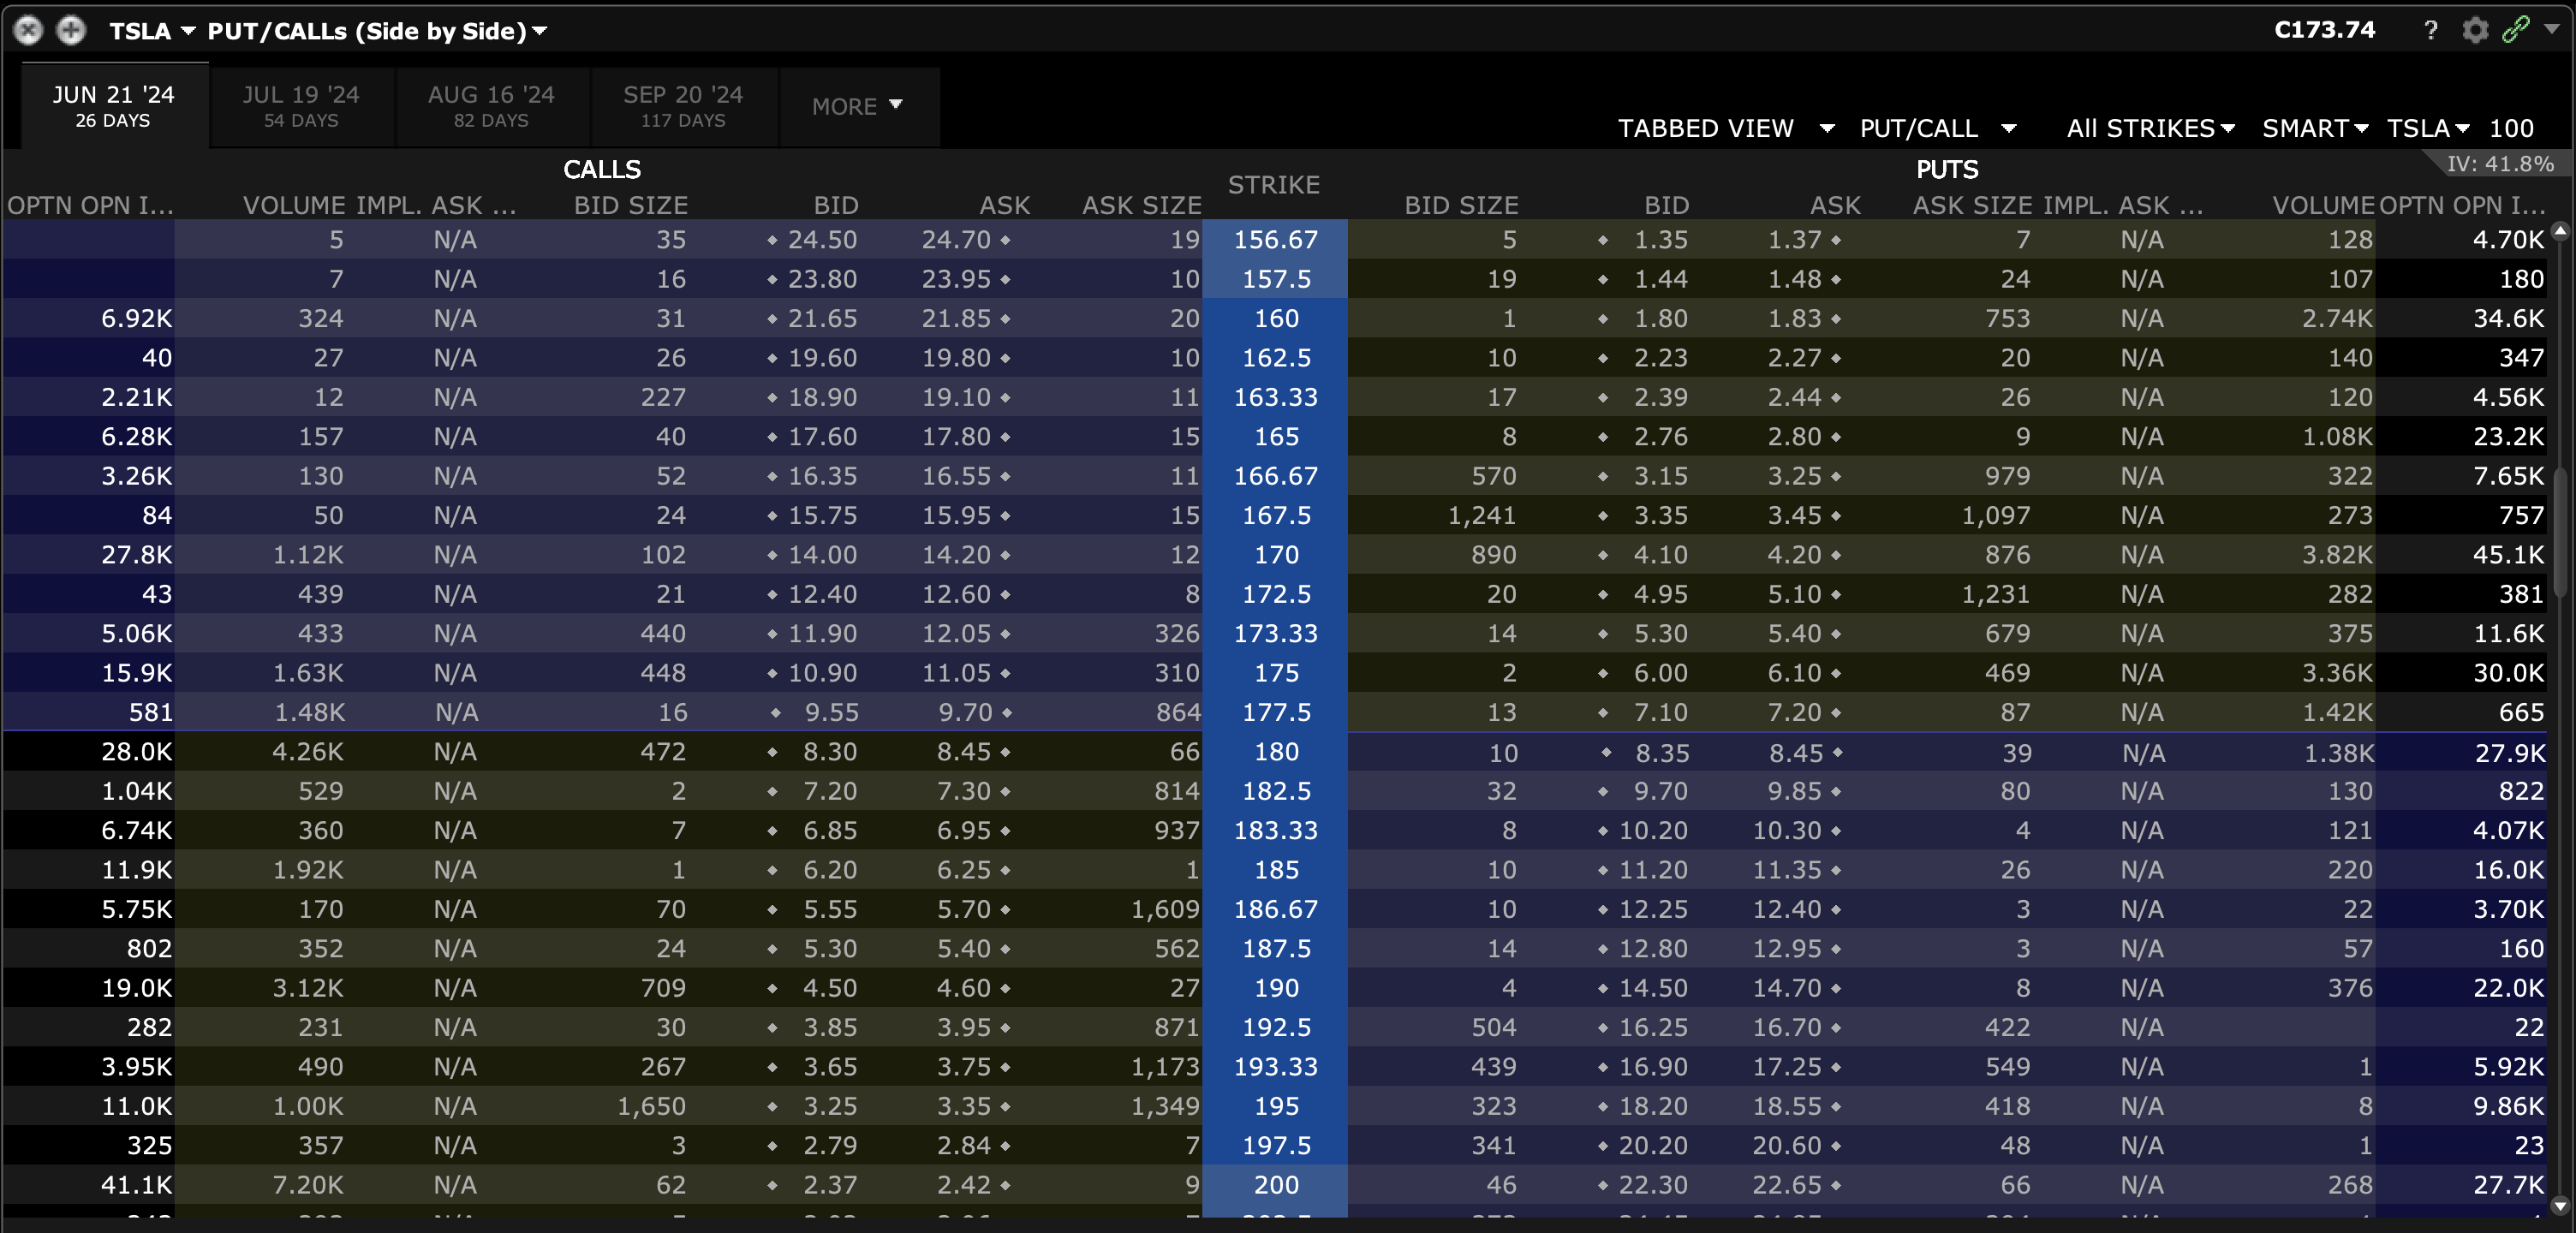
\includegraphics[scale=0.28]{img/option_chain.png}
        \caption{Option chain for TSLA viewed on May 26, 2024 at Interactive Broker's Trader Workstation (TWS). } 
        \label{fig:option_chain}
      \end{figure}
    \end{example}

    To accurately value this, the trader must have a good feel for both the directional movement of the market \textit{and} the timing. A equity trader just needs directional. 

  \subsection{Intrinsic Value and Time Premium}

    Let's try to construct some model for this price. The most obvious factor is the difference between the actual price and the strike price, which tells us if our option is currently profitable or not (if we exercised it now). 

    \begin{definition}[Intrinsic Value]
      The \textbf{intrinsic value} is simply what the holder of the option contract would make if they chose to exercise it. That is, for a long call option, it is 
      \begin{equation}
        \IV_K (t, T) = \max\{0, S_t - K\}
      \end{equation}
      and for a long put option, it is 
      \begin{equation}
        \IV_K (t, T) = \max\{0, K - S_t\}
      \end{equation}
      At some time $t$, if the value is positive, then the contract is \textbf{in-the-money (ITM)} or else it is \textbf{out-of-money (OTM)}. If $K = S_t$, then it is \textbf{at-the-money (ATM)}.\footnote{Technically, ATM options are the same at OTM, but as we will see later, ATM options have very specific and desirable characteristics, and such options tend to be the most actively traded. } However, since the strike prices are quantized (e.g. \$65, \$70, \$75, etc.), the contract with strike price closest to the underlying spot is known as the ATM. 
    \end{definition}

    With this, we can already draw \textit{payoff diagrams}, which show the intrinsic value of the option (i.e. the value of the option \textit{at expiry}). 

    \begin{example}[4 Basic Options: Payoff Diagrams at Expiry]
      The 4 basic sides of an option contract are listed below. 
      \begin{enumerate}
        \item If party \textbf{A} buys a call option from party \textbf{B}, then \textbf{A} is in a \textbf{long call} position and has the right to buy at the strike price. \textbf{B} is in a \textbf{short call} position and has the possible obligation to sell at the strike price. 

        \begin{figure}[H]
          \centering 
          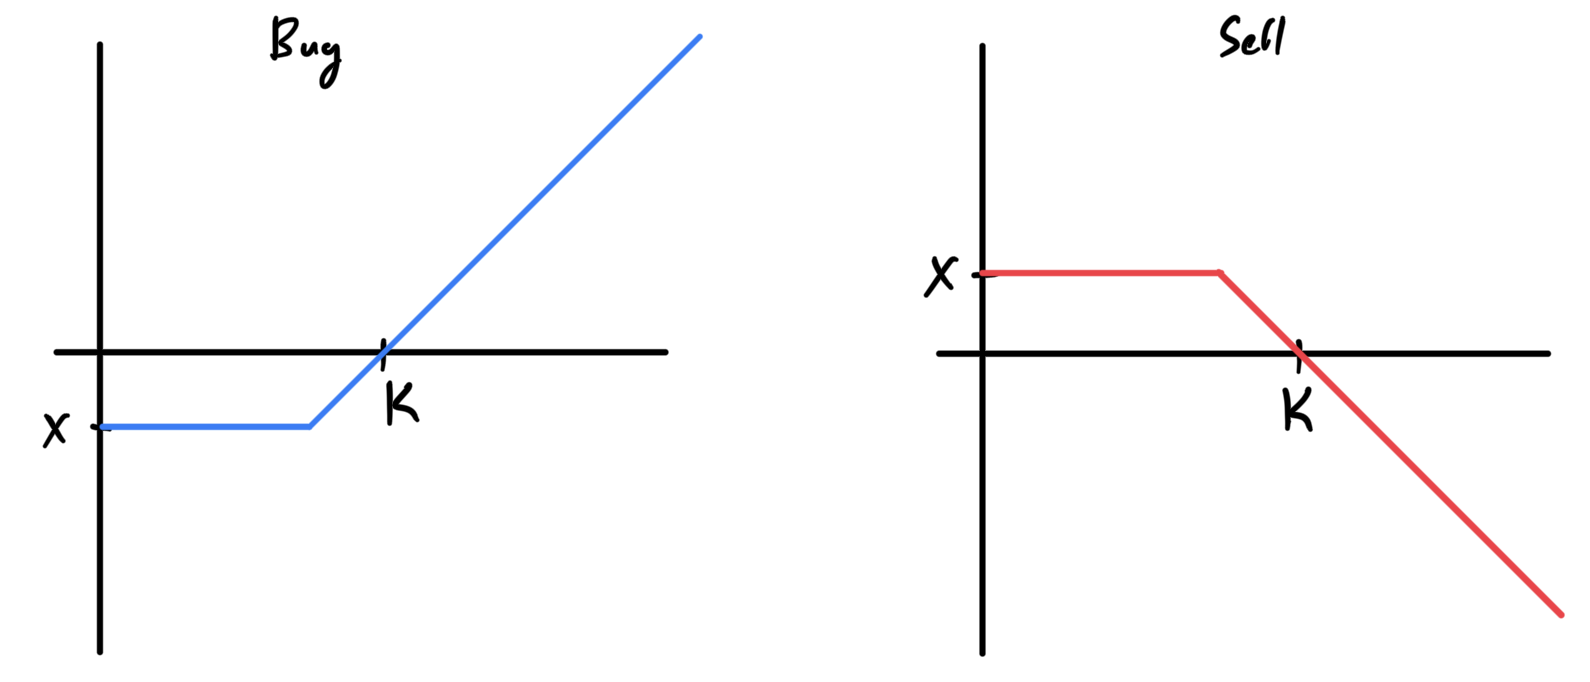
\includegraphics[scale=0.4]{img/call_options.png}
          \caption{For calls, the premium is higher as the strike price gets lower, since you can buy at lower prices. Note that the buyer has limited loss and has unlimited gain with the long put, while the seller has limited gain and unlimited loss with the short put.} 
          \label{fig:call_options}
        \end{figure}

        \item If party \textbf{A} buys a put option from party \textbf{B}, then \textbf{A} is in a \textbf{long put} position and has the right to sell at the strike price. \textbf{B} is in a \textbf{short put} position and has the possible obligation to buy at the strike price. 

        \begin{figure}[H]
          \centering 
          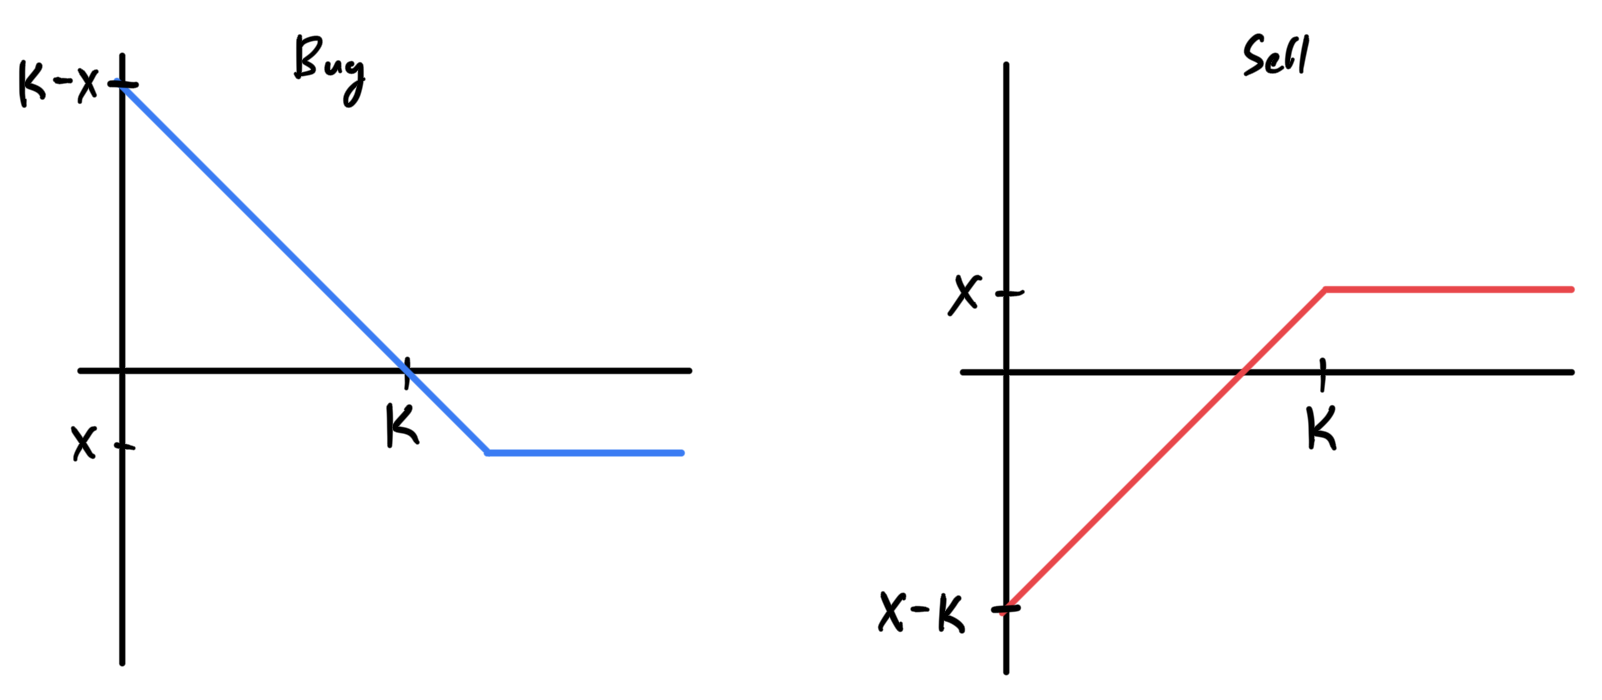
\includegraphics[scale=0.4]{img/put_options.png}
          \caption{For puts, the premium is higher as the strike price is higher, since you can sell at a higher price. Note that the buyer has limited loss and limited gain, and the seller also has limited loss and limited gain. } 
          \label{fig:put_options}
        \end{figure}
      \end{enumerate}

      There are already a few interesting properties. First, note that the long call and short put (like a double negative) take long positions in the underlying, and the other two short positions. 
    \end{example}

    With just the intrinsic value, two options with the same strike price, but with one expiring in 1 month and the other expiring in 6 months, must be worth the same. This is usually not what we see in the market, and the 6-month contract is worth more. Therefore, there is some time component as well. 

    \begin{definition}[Time value]
      The \textbf{time value} component $\TV_K (t, T)$ of an option takes into additional considerations: 
      \begin{enumerate}
        \item There is the probability of the underlying asset's price moving in or against our favor during the time remaining. This also has to do with the \textit{volatility} of this underlying spot price, which we will talk about later. 

        \item Traders are willing to pay this additional amount due to some protective characteristics offered by options than an outright long or short equity position. 
      \end{enumerate}
      It must clearly satisfy  
      \begin{equation}
        \lim_{t \rightarrow T} \TV_K (t, T) = 0
      \end{equation}
      However, there are times when the time value can be $0$, at which the contract is said to be trading \textbf{at parity}. 
    \end{definition}

    \begin{theorem}[Components of Options Premium]
      The premium paid for an option can be divided into two components, the intrinsic value and the time value. 
      \begin{equation}
        V_K(t, T) = \IV_{K} (t, T) + \TV_K (t, T)
      \end{equation}
      This must satisfy the following. 
      \begin{enumerate}
        \item The time premium must monotonically vanish at $t = T$, i.e. is a \textit{wasting asset}. 
          \begin{equation}
            \lim_{t \rightarrow T} \TV_K (t, T) = 0 \implies \lim_{t \rightarrow T} V_K (t, T) = \IV_K (t, T) 
          \end{equation}
        \item The value of an option with underlying value of $0$ always is also $0$. That is, if $S_T = 0$ (almost surely), then 
          \begin{equation}
            V_K (t, T)  = 0
          \end{equation}
      \end{enumerate}
    \end{theorem}

  \subsection{Covered Positions}

    Options are used to hedge a lot of positions. 

    \begin{definition}[Covered Call]
      
    \end{definition}


  \subsection{Black Scholes Pricing Formula}

    To construct a naive model of an option's value that takes into account both the intrinsic value and the time premium, we can first take the expected intrinsic value at expiry.\footnote{This is what Natenberg does in the theoretical pricing models chapter before introducing Black Scholes.} Then, by buying the option for the duration, you are forgoing the opportunity to invest it with interest rate $r$, leading to the \textit{theoretical value}, or the present discounted expected value, of the contract. 
    \begin{equation}
      V_K (t, T) = e^{-r (T - t)} \mathbb{E} [\IV_K(T, T)] 
    \end{equation}
    which reduces to $e^{-r (T - t)} \mathbb{E}_{S_T} [ \max\{S_T - K, 0 \}]$ for a call and $e^{-r (T - t)} \mathbb{E}_{S_T} [ \max\{K - S_T, 0 \}$ for a put. This makes sense, since it works first with the intrinsic value.  
  
    However, this model is lacking for the following reasons. 
    \begin{enumerate}
      \item We don't know the probability distribution of $S_t$. 
    \end{enumerate}

    The problems are modeled through the Black-Scholes model comes in, which is stated with the following PDE.

    \begin{definition}[Black Scholes PDE]
      The \textbf{Black-Scholes PDE} is the following. 
      \begin{equation}
        \frac{\partial V}{\partial t} + \frac{1}{2} \sigma^2 S^2 \frac{\partial^2 V}{\partial S^2} + r S \frac{\partial V}{\partial S} - rV = 0
      \end{equation}
    \end{definition}

    It has the following solution, which we will state now but will elaborate later. 

    \begin{definition}[Black-Scholes Option Pricing Formula]
      Given a call option, the \textbf{Black-Scholes} pricing formula states that 
      \begin{equation}
        V_K (t, T) = \mathcal{B}_t (K, T - t, S_t, r, \sigma) = \Phi(d_1) S_t - \Phi (d_2) K e^{-r (T - t)}
      \end{equation}
      where $r$ is some risk-free applicable interest rate, $\Phi$ is the normal CDF, $\sigma$ is the volatility of the underlying, and 
      \begin{equation}
        d_1 = \frac{\ln (S_t / K) + \big( r + \frac{\sigma^2}{2}\big) (T - t)}{\sigma \sqrt{T - t}} \text{ and } d_2 = d_1 - \sigma \sqrt{T - t}
      \end{equation}
    \end{definition}

    Black-scholes also allows us to draw payoff diagrams for time $t$ that is not necessarily at expiry, known as \textit{risk diagrams}. This allows us to see the value of these options both at different spot prices of the underlying and at different points in time. 

    \begin{figure}[H]
      \centering
      \begin{subfigure}[b]{0.48\textwidth}
      \centering
        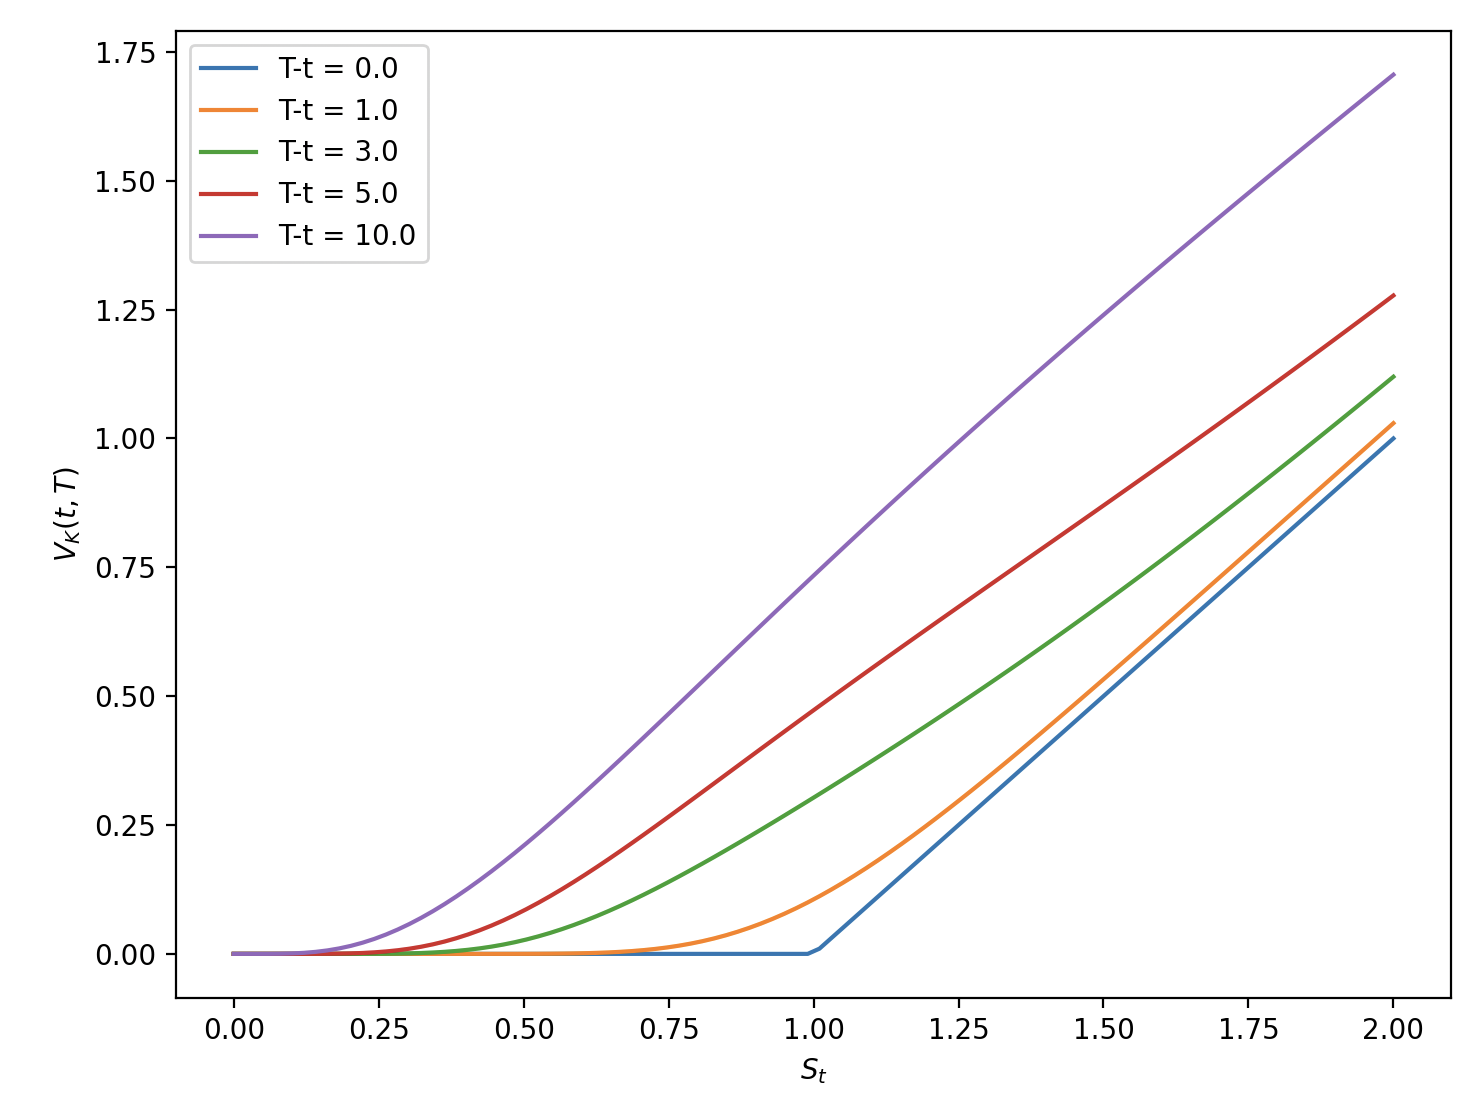
\includegraphics[width=\textwidth]{img/value_graph_over_time.png}
        \caption{The value graphs of European options over time according to Black Scholes model. }
        \label{fig:value_graph_over_time}
      \end{subfigure}
      \hfill 
      \begin{subfigure}[b]{0.48\textwidth}
      \centering
        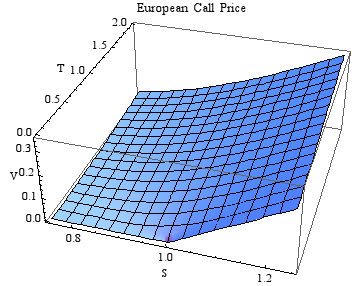
\includegraphics[width=\textwidth]{img/option_surface.png}
        \caption{3D surface. }
        \label{fig:option_surface}
      \end{subfigure}
      \caption{}
      \label{fig:option_pricing_graphs}
    \end{figure}
    
    \begin{figure}[H]
      \centering 
      \begin{lstlisting}
        import numpy as np 
        import math
        from scipy.stats import norm
        import matplotlib.pyplot as plt 

        def blackScholes(K:float, T_t:float, S_t:float, r:float, sigma:float) -> float: 
            d1 = (np.log(S_t / K) + (r + (sigma ** 2)/2) * (T_t)) / (sigma * math.sqrt(T_t))  
            d2 = d1 - sigma * T_t 
            return norm.cdf(d1) * S_t  - norm.cdf(d2) * K * math.e ** (-r * T_t)

        K = 1.0 
        r = 0.03
        sigma = 0.23
        X = list(np.linspace(0, 2, 100))
        for T_t in [0., 1., 2., 3.]: 
            Y = []
            for S_t in X: 
                Y.append(blackScholes(K, T_t, S_t, r, sigma))
            plt.plot(X, Y, label=f"{T_t}")
        plt.show() 
      \end{lstlisting}
      \caption{Code snippet used to generate graphs.} 
      \label{fig:black_scholes_graph_code}
    \end{figure}

  \subsection{Implied Volatility} 

    Therefore, to solve Black Scholes formula for the value, you really just need $K, T - t, S_t, r,$ and $\sigma$. The first four arguments are easy to find and has no ambiguity. The final volatility is a bit more slippery because it turns out that if you take the historical volatility and plug it into the Black-Scholes equation, you get a value that isn't too close to the actual current price. This can be attributed to many things, one being that the Black-Scholes model is not correct. While this is certainly a possibility, another one is to delve a bit deeper on what this difference means. The function $\mathrm{BS}$ is monotonically increasing w.r.t. $\sigma$, and so it is invertible. So, rather than looking at the difference in the output pricing, we can look at the difference in the volatility. 

    \begin{definition}[Implied Volatility]
      The \textbf{implied volatility} of an option is the theoretical volatility $\sigma$ of the underlying s.t. the Black-Scholes pricing model equals the current market price of the option. That is, taken $S_t, K, T, r$ to be constant, it is the value of $\sigma$ s.t. 
      \begin{equation}
        C_t = \mathcal{B}(K, T - t, S_t, r, \sigma)
      \end{equation}
      In essence, the implied volatility acts as the expected volatility of the stock during the time period from not $t$ until expiration $T$. The greater this implied volatility is, the more changes that the option will be ITM, and the higher value it will have. 
    \end{definition}

    Essentially, the implied vol is the public's general estimate of what the future realized vol will be. Therefore, the IV is the determinant of the price and the future realized vol is the determinant of the value. 

    \begin{enumerate}
      \item If the implied volatility is greater than the historical volatility, this means that current prices are overestimating the volatility of the underlying. This overestimation of $\sigma$ means that the option premium is overvalued, and we might likely see a drop in option prices. 
      \begin{equation}
        V_K (t, T) = \mathcal{B} (K, T - t, S_t, r, \sigma) < C_t
      \end{equation}

      \item If it is less, then current prices are underestimating it, meaning that the option is undervalued. 
      \begin{equation}
        V_K (t, T) = \mathcal{B} (K, T - t, S_t, r, \sigma) > C_t
      \end{equation}
    \end{enumerate}

    Surprisingly, it turns out that most of the time, the IV is greater than historical volatility, a phenomenon we will explain now. 

    \begin{definition}[Volatility Risk Premium]
      The \textbf{volatility risk premium} refers to the following two phenomena, which are equivalent due to monotonicity of $\mathcal{B}$ w.r.t. $\sigma$. 
      \begin{enumerate}
        \item Implied volatility tends to exceed realized volatility of the same underlying asset over time. 
        \item The market price $C_t$ of the option tends to exceed the Black-Scholes pricing $\mathcal{B}(K, T - t, S_t, r, \hat{\sigma})$, where $\hat{\sigma}$ is the historical volatility. 
      \end{enumerate}
    \end{definition}

    The cause for this is still up for debate, but a study from Yale suggests that market participants tend to overestimate the probability of a significant crash, leading to higher demand for options. This heightened perception of risk may lead to higher willingness to pay for these options to hedge a portfolio, which is realized in the additional premium $C_t - \mathcal{B}(K, T - t, S_t, r, \hat{\sigma})$. 

    This is quite weird, but it gets even weirder. Let us have two options with the same expiry $T$, same underlying asset $S_t$, same interest rate (of course, since this is dependent on the environment), but different strike prices $K^1$ and $K^2$. The volatility should be the same between the two options since they have the same underlying. Therefore, the difference in their prices should be accounted purely from the difference in their strikes. 
    \begin{equation}
      C_t^1 \neq C_t^2 \implies K^1 \neq K^2
    \end{equation}
    Great, so for a given moment in time $t$, let's take a look at all the options of a certain common underlying and their strike prices $K$. Their prices $C_t^i$ should be different, and if we calculate the implied volatility for each strike $K$, we \textit{should} get the same estimate of volatility. 

    \begin{figure}[H]
      \centering 
      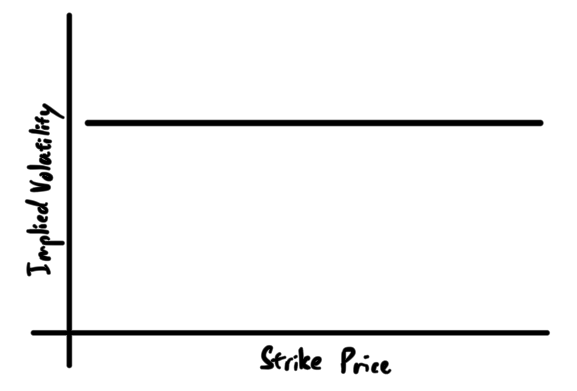
\includegraphics[scale=0.4]{img/expected_vol_graph.png}
      \caption{What we expect our strike price vs implied volatility graph to look like for a collection of options. } 
      \label{fig:expected_volatility_graph}
    \end{figure}

    \begin{definition}[Volatility Smile]
      Empirically, this is not the case, and we see a \textbf{volatility smile} centered around ATM. This means that ATM options have lower implied volatility than OTM or ITM options. Therefore, as the strike price moves away from the current stock price, the price of the options are in fact higher than what is accounted for in the Black-Scholes model, meaning that they are overvalued.  
      \begin{figure}[H]
        \centering 
        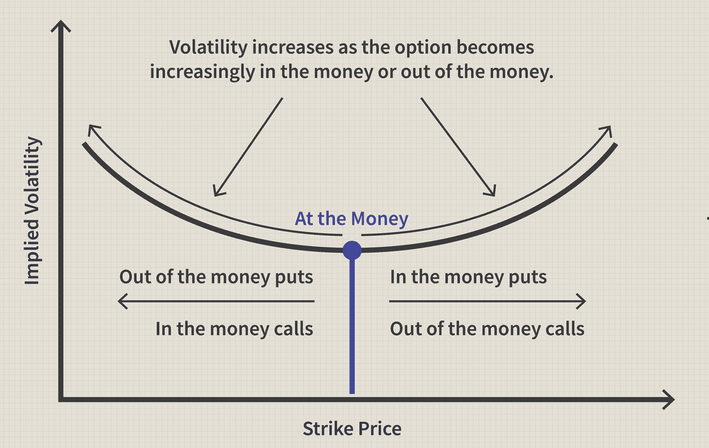
\includegraphics[scale=0.4]{img/vol_smile.png}
        \caption{Volatility smile} 
        \label{fig:vol_smile}
      \end{figure}
    \end{definition}

    However, this may not be symmetrical. 

    \begin{definition}[Volatility Skew/Smirk]
      
    \end{definition}

  \subsection{The Greeks}

    \begin{definition}[Delta]
      The \textbf{delta} is the rate of change of the value w.r.t. the price of the underlying security. 
      \begin{equation}
        \Delta_t \coloneqq \frac{\partial V_K (t, T)}{\partial S_t}
      \end{equation}
      meaning that for every \$1 increase in stock price, the option price increases roughly by \$$\Delta$, with all else being equal. It indicates how many options contracts are needed to hedge a long or short position in the underlying asset. Note that the delta for a call must be in $[0, 1]$ and of a put must be in $[-1, 0]$, but traders tend to describe it in $[0, 100]$ and $[-100, 0]$. 
    \end{definition}

    \begin{definition}[Gamma]
      The \textbf{gamma} is the sensitivity of $\Delta$ w.r.t. $S$, i.e. the double derivative. 
      \begin{equation}
        \Gamma_t \coloneqq \frac{\partial^2 V_K (t, T)}{\partial S_t^2}
      \end{equation}
    \end{definition}

    \begin{theorem}[Delta and Gammas as Time Passes]
      
    \end{theorem}

    \begin{definition}[Theta]
      The \textbf{theta} measures the impact of a change in time remaining. 
      \begin{equation}
        \Theta_t \coloneqq \frac{\partial V_t}{\partial t}
      \end{equation}
    \end{definition}

    \begin{definition}[Rho]
      The \textbf{rho} measures the impact of a change in interest rates. 
      \begin{equation}
        \rho_t \coloneqq \frac{V_K (t, T)}{\partial r}
      \end{equation}
    \end{definition}

    \begin{definition}[Vega]
      The \textbf{vega} measures the impact of a change in the volatility of the underlying. 
      \begin{equation}
        \nu_t \coloneqq \frac{\partial V_K (t, T)}{\partial \sigma}
      \end{equation}
    \end{definition}

  \subsection{Put Call Parity}

\section{Dynamic Hedging}

\section{Spreading}

\section{Forward Rates and Libor}

  One might want to borrow money at a future time, say from $T_1$ to $T_2$, but they are not sure what the interest rate will be. Therefore, they can buy a forward contract that expires at $T_1$, with an underlying zero coupon bond that has maturity of $T_2$. This essentially allows them to lock in the interest rate $r_{T_1, T_2}$ for a future loan between $T_1$ and $T_2$. This is called the \textit{forward rate}. 

  \begin{definition}[Forward Rate]
    The \textbf{forward rate} at current time $t$ for period $T_1$ to $T_2$ ($t \leq T_1 \leq T_2$) is the interest rate (agreed at $t$) at which one can borrow or lend money from $T_1$ to $T_2$, i.e. the interest rate $r_{T_1, T_2}$. 

    \begin{figure}[H]
      \centering 
      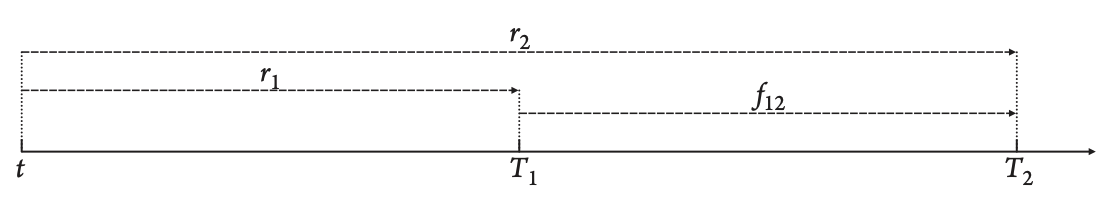
\includegraphics[scale=0.35]{img/forward_zero_rates.png}
      \caption{Letting $r_1$ be the interest rate from $t$ to $T_1$ and $r_2$ be the interest rate from $t$ to $T_2$, we can see that the forward rate $f_{12} = r_{T_1, T_2}$ is the interest rate from $T_1$ to $T_2$.}
      \label{fig:forward_zero_rates}
    \end{figure}
  \end{definition}

  A simple replication argument gives the following result about the forward rate. 

  \begin{theorem}[Forward Rate]
    At time $t$, the fair value of the forward rate $f_{12}$ is given by 
    \begin{equation}
      f_{12} = \frac{(r_2 (T_2 - t) - r_1 (T_1 - t))}{T_2 - T_1}
    \end{equation}
    if the rates of continuously compounded and 
    \begin{equation}
      f_{12} = \bigg( \frac{(1 + r_2)^{T_2 - t}}{(1 + r_1)^{T_1 - t}} \bigg)^{\frac{1}{T_2 - T_1}} - 1 
    \end{equation}
  \end{theorem}
  \begin{proof}
    By the replication argument, consider two portfolios A and B with the same money at time $t$. A first borrows money at the rate $r_1$ and then at the forward rate $f_{12}$, and B borrows at the rate of $r_2$. Then, the value of the two portfolios must be the same at time $T_2$, and so we have 
    \begin{equation}
      e_{r_1(T_1 - t)} e_{f_{12}(T_2 - T_1)} = e_{r_2(T_2 - t)} \implies f_{12} = \frac{(r_2 (T_2 - t) - r_1 (T_1 - t))}{T_2 - T_1}
    \end{equation}
    and if they are discretely compounded we have 
    \begin{equation}
      (1 + r_1)^{T_1 - t} (1 + f_{12})^{T_2 - T_1} = (1 + r_2)^{T_2 - t} \implies f_{12} = \bigg( \frac{(1 + r_2)^{T_2 - t}}{(1 + r_1)^{T_1 - t}} \bigg)^{\frac{1}{T_2 - T_1}} - 1
    \end{equation}
  \end{proof}

  \begin{theorem}[Forward Price of Zero Coupon Bonds]
    For $T_1 \leq T_2$, consider a forward contract with maturity $T_1$ on a ZCB with maturity $T_2$. That is, the underlying asset price is $S_t = Z(t, T_2)$. Then, the forward price, i.e. the price where one can (for no cost) agree to buy a forward contract on the $T_2$-ZCB with a expiry date of $T_1$, is 
    \begin{equation}
      F(t, T_1, T_2) = \frac{Z(t, T_2)}{Z(t, T_1)}
    \end{equation}
  \end{theorem}
  \begin{proof}
    Let 
    \begin{enumerate}
      \item Portfolio A be one ZCB maturing at $T_2$. 
      \item Portfolio B be one long forward with delivery price $K$, and $K$ ZCBs maturing at $T_1$. 
    \end{enumerate}
  \end{proof}

  \begin{corollary}
    Since the value of a ZCB with annually compounded rate is 
    \begin{equation}
      Z(t, T_i) = \frac{1}{(1 + r_i)^{T_i - t}} \text{ for } i = 1, 2
    \end{equation}
    we can substitute to see that the forward price of a ZCB is 
    \begin{equation}
      F(t, T_1, T_2) = \frac{Z(t, T_2)}{Z(t, T_1)} = \frac{(1 + r_1)^{T_1 - t}}{(1 + r_2)^{T_2 - t}} = \frac{1}{(1 + f_{12})^{T_2 - T_1}}
    \end{equation}
  \end{corollary}

\section{Exercises}

  \begin{exercise}[Hull 1.3]
    What is the difference between entering in to a long forward contract when the forward price is $\$50$ and taking a long position in a call option with a strike price of $\$50$? 
  \end{exercise}
  \begin{solution}
    The answer is clear when we look at the payoff graph for each one.  
    \begin{enumerate}
      \item The first difference is that the forward contract renders both parties obligated to buy or sell the underlying at a future time, while the option only gives the seller the obligation to sell, if the buyer requests it.  
      \item The second is that money is paid to enter into the options contract by the buyer, while the forward contract does not. 
      \item Both profits/losses are unlimited in the forward contract, while in the options contract, the buyer has limited loss and the seller has unlimited loss. 
      \item By having the safety of a limited downside for the call options buyer, they get a slightly lower payoff $S_T - C_0$ compared to the forward contract, which is $S_T$. Therefore, the options buyer doesn't actually make a profit until the price of the underlying asset is at least $C_0 + K$. 
      \item If $S_T > K$, we would wish we were taking the forward, and if $S_T < K$, then we wish we were taking the call option.  
    \end{enumerate}
    \begin{figure}[H]
      \centering 
      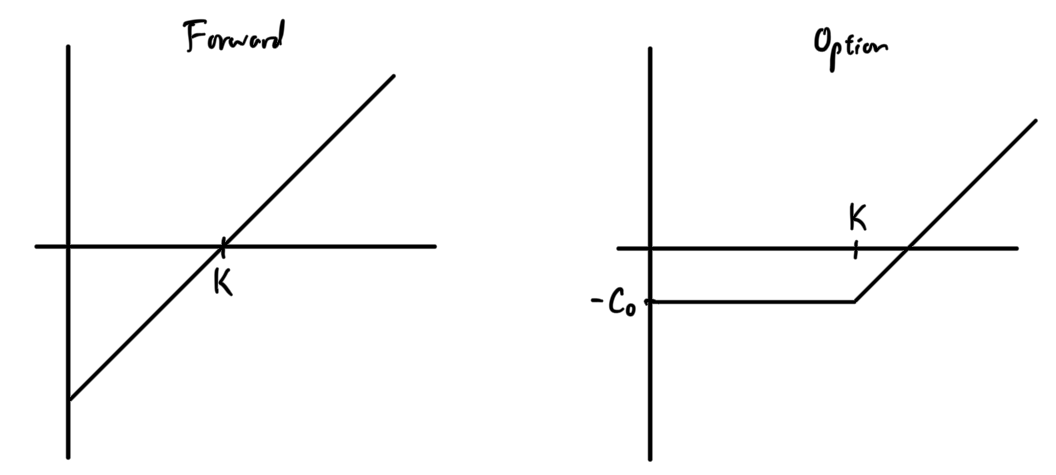
\includegraphics[scale=0.4]{img/ex1-3.png}
      \caption{The payoff graph for the forward contract and the call option from the buyers side.} 
      \label{fig:ex1-3}
    \end{figure}
  \end{solution}

  \begin{definition}[Pips]
    For the next problem, it helps to know that a \textbf{pip} is 1/100 of a cent. 
  \end{definition}

  \begin{exercise}[Hull 1.5]
    An investor enters into a short forward contract to sell $100,000$ British Pounds for US dollars at an excahnge rate of $1.5$ dollars per pound. How much does the investor gain or lose if the exchange rate at the expiration date is $1.4900$ dollars per pound? What if it is $1.5200$ dollars per pound? 
  \end{exercise}
  \begin{solution}
    Note that we must specify the currency of the profit or loss. It turns out that the payoff will always be in the currency that the investor is selling. The investor is selling the forward, so they are obligated to sell it at $1.5000$ dollars per pound. 
    \begin{enumerate}
      \item If the rate is $1.4900$, then the investor sells the pounds for $150,000$ USD and can buy a little bit more than $100,000$ pounds. In fact, they are making a profit of $100,000 \cdot 0.0100 = 1,000$ dollars.
      \item If the rate is $1.52$, then the investors sells the pounds for $150,000$ USD and can buy a little less than $100,000$ pounds, so they lose $100,000 \cdot 0.0200 = 2,000$ dollars. 
    \end{enumerate}
  \end{solution}


  \begin{exercise}[Hull 1.6]
    A trader enters into a short cotton futures contract when the futures price is 50 cents per pound. The contract is for the delivery of 50,000 pounds. At the end of the contract, the price of cotton is $48.20$ or $51.30$ per pound. What is the trader's gain or loss?
  \end{exercise}
  \begin{solution}
    The trader is selling the cotton, and the buyer is obligated to buy. Therefore, 
    \begin{enumerate}
      \item the trader makes $(50 - 48.20) \cdot 50,000 = 1.8 \cdot 50,000 = 90,000$ cents, or $\$900$ if the price is $48.20$. 
      \item the trader loses $(51.30 - 50) \cdot 50,000 = 1.3 \cdot 50,000 = 65,000$ cents, or $\$650$ if the price is $51.30$.
    \end{enumerate}
  \end{solution}

  \begin{exercise}[Hull 1.16]
    A trader writes (sells) a December put option with a strike price of $\$30$. The price of the option is $\$4$. Under what circumstances does the trader make a profit? 
  \end{exercise}
  \begin{solution}
    Even without a payoff graph, we can see that since I'm selling the option, I'm getting $\$4$. Now, I'm obligated to buy the asset (since it's a put) at $\$30$, and therefore I will profit if the price of the asset is above $\$30$. However, since I already have the cushion of $\$4$, I'm really profiting if the asset price $S_T > 26$. 
    \begin{figure}[H]
      \centering 
      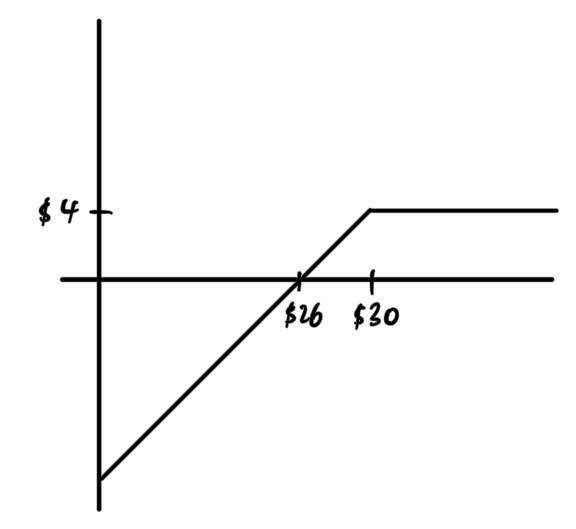
\includegraphics[scale=0.2]{img/ex1-16.png}
      \caption{The payoff graph for the put option from the sellers side.} 
      \label{fig:ex1-16}
    \end{figure}
  \end{solution}

  \begin{exercise}[Hull 1.22]
    I am in a long forward contract and a long put option at the same strike price $K$. What is the payoff of this position at expiration?
  \end{exercise}
  \begin{solution}
    You can simply draw the profit-loss diagram. 
    \begin{figure}[H]
      \centering 
      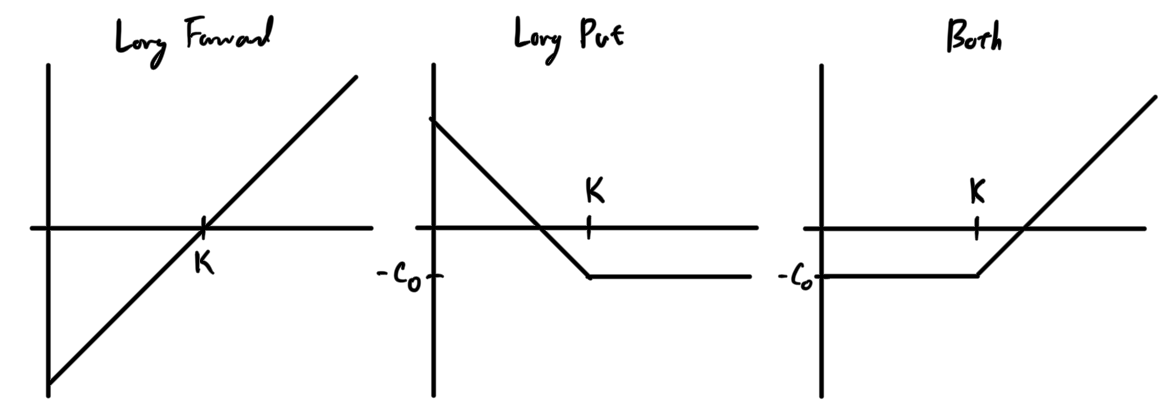
\includegraphics[scale=0.2]{img/ex1-22.png}
      \caption{The payoff graph for the long forward and long put option at the same strike price.} 
      \label{fig:ex1-22}
    \end{figure}
  \end{solution}

  \begin{exercise}[Hull 1.23]
    We have a \textbf{Index Currency Option Note (ICON)} which states the following: 
    \begin{enumerate}
      \item If the exchange rate USD.JPY $ < 169$, then the bond pays $1000$ USD.
      \item If $84.50 \leq USD.JPY \leq 169$, then the bond pays 
        \begin{equation}
          1000 - \max\bigg\{ 0, 1000 \Big( \frac{169}{S_T} - 1 \Big)\bigg\}
        \end{equation}
      \item If $USD.JPY < 84.50$, then the bond pays nothing. 
    \end{enumerate}
    Show that this ICON is a combination of a bond and two options. 
  \end{exercise}
  \begin{solution}
    This seems a bit easy since we can draw the payoff diagram as such. 
    \begin{figure}[H]
      \centering 
      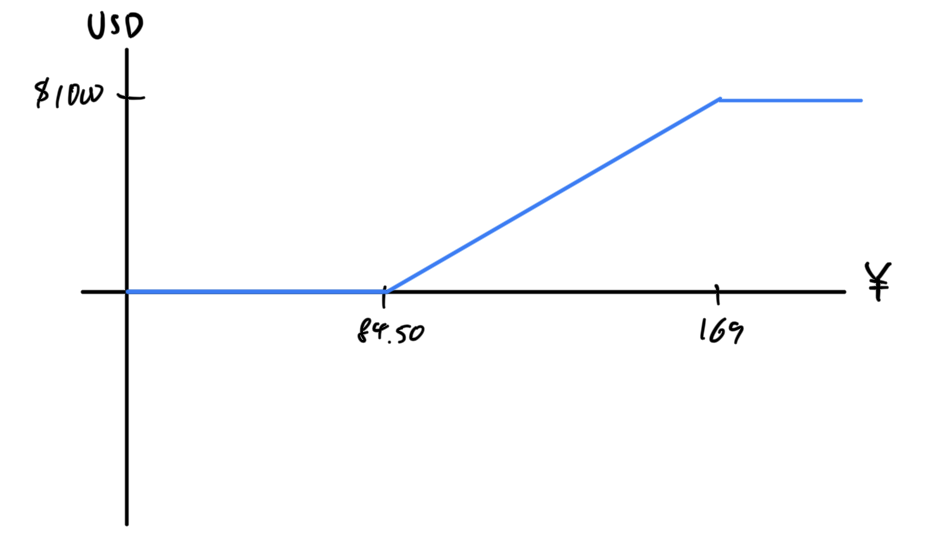
\includegraphics[scale=0.2]{img/ex1-23-1.png}
      \caption{} 
      \label{fig:ex1-23-1}
    \end{figure}
    However, the underlying asset is shown in yen and the payoff in USD, which complicates calculations. You should rather change the underlying to be USD by changing USD.JPY to JPY.USD. Then, we can do some quick sketches to find that you should have a 
    \begin{enumerate}
      \item Bond at $\$1000$. 
      \item Short call at $1/169$ for $\$1000$. 
      \item Long call at $1/84.50$ for $\$1000$.
    \end{enumerate}
    \begin{figure}[H]
      \centering 
      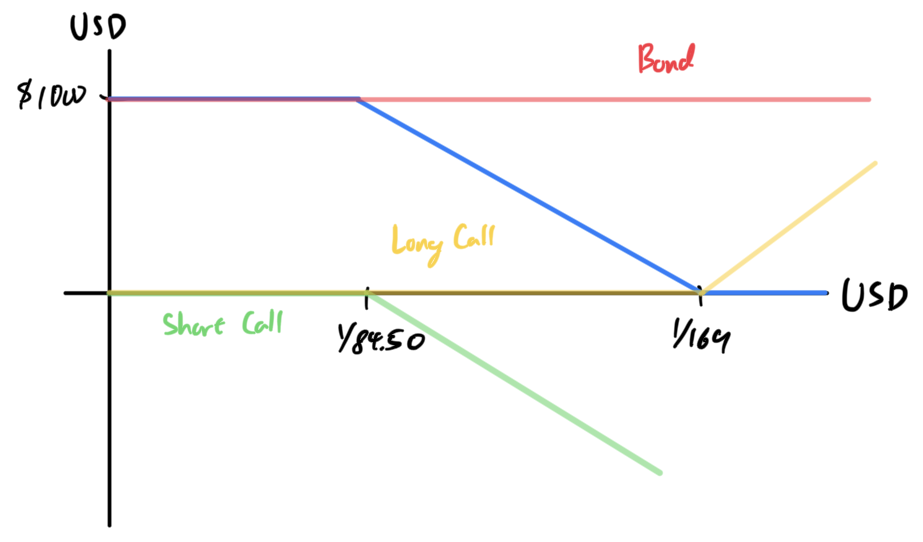
\includegraphics[scale=0.2]{img/ex1-23-2.png}
      \caption{} 
      \label{fig:ex1-23-2}
    \end{figure}
  \end{solution}

\section{Appendix}

  Futures are mostly cash settled (e.g. look at futures on SP500 index. you can't deliver fractional shares. )

  Margin calls with futures. 

  The difference between the spot and the futures price is called the basis gap/risk. They tend to converge as we approach the expiration date. 

  Order types (market, limit - default, stop), which exists for both long and short futures. 

  Regulations are done by the CFTC (Dodd-Frank Act expands CFTC oversight to OTC markets due to 2008). Accounting (does unrealized gains count as taxable income?) and taxes can be country specific. 

  Talk about derivatives in general 
  - stuff like payoff graphs 
  - definitions of derivatives 

  Forwards \& Futures 
  - how they work, with trading, delivery, quality of goods, settlement (delivery or cash settled). Does delivery actually happen? You must actually request to have it delivered to a warehouse you set up. This could have inventory/delivery fees as well.  
  - basis risk (spot price of asset $A$ is $S_A$, and the futures is $F_A$). (8)
  - hedging strategies with futures (short \& long futures) hedge ratio, with cross-hedging, and minimizing the variance of our position. (is this delta-hedging?) 
  - stock index futures (you need CAPM to evaluate this)




\end{document}
